\documentclass[12pt, a4paper]{article}  %% is it okay to change to 12 for readability?
\setlength\parindent{24pt}

\usepackage{mlt-thesis-2015}

% With Xetex/Luatex this shouldn't be used
%\usepackage[utf8]{inputenc}

\usepackage[polish, english]{babel}
\usepackage [autostyle, english = american]{csquotes}
\MakeOuterQuote{"}
%%\usepackage[T1]{fontenc}
\renewcommand\polishtablename{Table}
\renewcommand\polishfigurename{Figure}
\renewcommand{\contentsname}{Contents}
\usepackage{graphicx}
\usepackage{caption}
\usepackage{subcaption}
\usepackage{multirow}
\usepackage{makecell}
\usepackage{float}
\restylefloat{table}
\usepackage{longtable}
\usepackage{tipa}

\usepackage{setspace}
\usepackage{subfiles} 
\usepackage{hyperref}
\usepackage{booktabs}
\graphicspath{ {figures/} }

\hypersetup{
colorlinks,
allcolors={blue}
}


\title{\textit{A catchy title}}  %% come up with a better title!
\subtitle{An exploration of the computational methods for \\ identifying language variation in Polish}
\author{Maria Irena Szawerna}

\begin{document}

%% ============================================================================
%% Title page
%% ============================================================================
\begin{titlepage}

\maketitle

\vfill

\begingroup
\renewcommand*{\arraystretch}{1.2}
\begin{tabular}{l@{\hskip 20mm}l}
\hline
Master's Thesis: & 30 credits \\
Programme: & Master’s Programme in Language Technology\\
Level: & Advanced level \\
Semester and year: & Spring, 2023 \\
Supervisor: & Aleksandrs Berdicevskis \\
Examiner: & Asad Sayeed \\ %% make sure that titles are not needed
Keywords: & language variation, Polish, diachronic linguistics %% can come up with better examples!
\end{tabular}
\endgroup

\thispagestyle{empty}
\end{titlepage}

%% ============================================================================
%% Abstract
%% ============================================================================
\newpage
\singlespacing
\section*{Abstract}

\textbf{WRITE AT THE END}

This is a template for master theses within the MLT programme at GU. The original author is Richard Johansson. It has since then been updated by Simon Hengchen. Questions (not compilation errors please, especially not the day before the deadline) should be addressed to \texttt{simon.hengchen@gu.se}.

The ACL anthology\footnote{\url{https://aclanthology.org/}} provides canonical, recommended bibtex entries. Prefer these to those you find on Google Scholar or dblp or anywhere else. The official ACL anthology bibtex is included within this template (see bottom of \texttt{main.tex}), and if you use Overleaf to compile this template you can update the \texttt{anthology.bib} file automatically (click on it, then click "refresh."). Should you want to cite papers not included in the ACL anthology, insert the bibtex entries in \texttt{personal.bib}. It is also included at the bottom of \texttt{main.tex}, and populated with some entries of work by GU researchers/some works you might find useful, e.g.

Please compile this document with Xetex/Luatex. PDFLaTeX will also work, but in that case make sure that \texttt{utf-8} is enabled (line 6 of \texttt{main.tex}.) With Xetex/Luatex, weird Swedish characters such as "å" will work out of the box, you will not have to include them using e.g. ``\texttt{\textbackslash aa}.''

The structure below is but a suggestion. Add/remove sections as you see fit.

\thispagestyle{empty}

%% ============================================================================
%% Preface
%% ============================================================================
\newpage
\section*{Preface}

This thesis would not have taken shape without a number wonderful people, and I would like to take some time to thank them all.  

I would like to thank my supervisor, Sasha Berdicevskis, for believing in the initial idea I had and for guiding me through many of the decisions that shaped the thesis into what it is today, as well as for showing me that I need not forsake my love of historical linguistics even in this program.

I will forever be grateful to the rest of the teachers and staff of the MLT program, who have taught me so many of the skills that I put to test while working on this topic, but also many more that I will hopefully utilize in the future. I am also happy to have met all the wonderful people that I studied with throughout these two years. I cannot wait to see what future lies ahead of us!

I want to extend my deepest thanks to my family members who were involved in procuring of the historical data: my grandfather, Piotr Kociatkiewicz, who meticulously transcribed our mutual ancestor's memoir from scans provided by my aunt Anna Chodorowska. It was my grandfather's question whether he should standardize the spelling of the text that sparked my interest in it as a linguistic resource - and without that question and the endeavor to transcribe the memoir, this thesis would not have been written.

I am also deeply grateful for the time and help given to me by dr hab. Piotr Pęzik, who not only made it possible for me to access the National Corpus of Polish (NKJP), but also took his time to explain to me its ins and outs.

I want to thank all of my friends and family whose support and faith in me carried me through the ups and downs: my father, Michał Szawerna, for his eagerness to discuss all things lingustics with me; my grandmother, Ewa Wajda-Kociatkiewicz, for her faith in me; my partner, Tobias Ström, for his patience and for believing in me at times when I did not believe I could finish this degree; my friends - Tomek Kos, Kasia Kuśmierczyk, Jakub Wróbel, Piotrek Szulc, Sandra Kierasińska, Freja Edvardsson, and so many others - for their unwavering support and friendship, despite some of us being hundreds of kilometers apart.

Finally, I hope that my mother, Justyna Kociatkiewicz, would be proud to see how far I have made it - and that she would be happy to see that her love for our family history persists in this thesis.

\thispagestyle{empty}

%% ============================================================================
%% Contents
%% ============================================================================
\newpage

\begingroup
\hypersetup{linkcolor=black} % This ensures that ONLY the ToC has black links
\begin{spacing}{0.0}
\tableofcontents
\end{spacing}
\endgroup

\thispagestyle{empty}

%% ============================================================================
%% Introduction
%% ============================================================================
\newpage
\setcounter{page}{1}

\section{Introduction}
\label{sec:intro}

While easy to overlook at the first glance, language variation plays a hugely important role in natural language processing: natural language as used by speakers is ever-changing, and NLP tools have to, to some extent, account for even the synchronic variation. As \citet{Zampieri2020NaturalLP} point out, developing methods to handle language variation is also relevant for adapting the existing tools to minority languages or dialects. While there are methods that allow for the utilization of raw data, \citet{ponti_2019} remarks that other methods still rely on annotated data which is difficult to come by for less popular languages. Simultaneously, as \citet{quantitative-historical} note, historical linguistics on its own is a data-driven field, and access to as well as methods for processing that data are very important; simultaneously, they highlight the usefulness of annotated corpora. This annotation may be especially useful when it comes to languages with a richer morphology, such as Slavic languages, as it may enable e.g. searching for all the inflectional forms of a given word \citep{pęzik_2012}. Thus, identifying the kinds of variation that occur between two languages or dialects not only constitutes a contribution to the body of knowledge about those languages on its own, but also opens up possibilities for adapting existing tools for major languages to be used for the partial automatizing of data annotation. 

\subsection{Research Questions}
\label{subsec:research-questions}

The aims of this thesis can be described as two sides of the same coin, as it seeks to simultaneously answer the following two questions:
\begin{enumerate}
    \item \textit{Is it possible to identify language variation in terms of orthography, morphology, and syntax in a Polish text using tools such as lemmatizers, POS-taggers, and modern corpora?}
    \item \textit{In what ways does the text in question, a 19\textsuperscript{th}-century memoir by Juliusz Czermiński, differ from modern Polish?}
\end{enumerate}

\subsection{Motivation}
\label{subsec:motivation}

As mentioned at the start of this section, investigating language variation is not only its own field of linguistics, but is also relevant for NLP - and methods and discoveries within these fields can inform each other. It is interesting to see how tools intended for working with modern languages can be used to identify ways in which those differ from their historical counterparts. These differences can help inform the pre-processing of the texts or ways in which the tools need to be adapted to enable a more reliable data annotation, which, in turn, can be used for further qualitative, corpus-based inquiries into some historical form of a language. 

Simultaneously, language variation is not only a thing of the past, but a continuous process which may lead to the modern tools becoming outdated in the future; furthermore, language varies also based on factors other than time, such as geography or social class, and this variation can also prove problematic to NLP applications. While methods such as cross-linguistic transfer learning do exist, they cannot be applied to all the tools equally, especially non-neural ones or ones that are not available for fine-tuning.

While the major focus of this thesis is on exploring historical language variation in Polish alongside the methods that can be employed for such investigations, hopefully it can yield insights into and spark some discussion about related topics, such as the handling of linguistic variation in NLP, computational methods in historical linguistics, as well as resources for historical linguistics and the annotation thereof.

\subsection{Contributions}
\label{subsec:contributions}

Within this thesis, a variety of ways for discovering historical linguistic variation using tools aimed for modern languages is tested. The methods are reviewed with regard to the kind results that they yield and the amount of annotation or preparation needed. While the majority of the methods do require the data to be annotated, some quite interesting observations can be made based on the results. Simultaneously, due to the nature of the experiments, the thesis unwittingly conducts a comparison of the performance of multiple tools (part-of-speech taggers and lemmatizers) on modern data, which can inform the choice of a tool for other research or real-life application. The manually annotated data that this project is centered around constitutes a non-negligible contribution to the body of annotated historical data for Polish. Finally, certain issues raised throughout the thesis can hopefully contribute to the discussion concerning the tagsets used for annotating data in Polish and certain biases present in the data.

\subsection{Scope}
\label{subsec:scope}

It is important to note that the data used in this project is not very big, and it does originate from a single author. Therefore, instead of trying to make claims about the language of the time and region, the focus is laid on the author's particular idiolect. At the same time, there likely are many more methods that could be used, directly or indirectly, for identifying language variation. In addition, some levels at which language can differ (phonology, pragmatics) are ommitted enitrely, and some are not discussed as in depth as others. Instead, the project focuses on the aspects detailed in \autoref{subsec:research-questions}. 

%% TODO:
% write motivation
% proofread subsection 3
% etc

%% ALREADY DONE:
% write xyz
% fixed bibtex
% etc

%% You can add and edit these comments as you see fit for the other sections, or use some other tool

\newpage

\section{Background and Related Work}
\label{sec:background}
% subsections are \subsection{title}
%% subssubsections are \subsubsection{title}
%% numbering will work automatically 

\subsection{The history of Polish (19\textsuperscript{th}-century)}
\label{subsec:history-pl}

When discussing a historical variant of a language it is important to situate it in the context of what is known about the history of that language in general. Historical grammars and descriptions are available for many of the major languages, and Polish is no exception --- although recently some concerns have been raised; \citet{dunaj_19} states that some of the most thorough descriptions of the history of Polish may be outdated given more recent research, and therefore in need of being updated. Nevertheless, much of the general information from these sources remains relevant and can be supported by more recent publications.

In what is considered to be one of the core texts of the study of historical Polish, \citet{klemensiewicz_76} describes the development of that language from mid-12\textsuperscript{th} century. Throughout the book, the author adopts the following periodization of the language\footnote{This periodization appears to be motivated by historical events such as the turning point between the Middle Ages and the Renaissance (1500s), the Enlightenment and the partitioning of Poland (late 1700s), the start of the Second World War (1939).}: Old Polish (until 1500s), Middle Polish (from 1500s to 1780s), New Polish (from 1780s to 1939), with no information provided about the period between 1939 and the modern times; however, it is worth pointing out that the book was written in 1976, and the author claims that the changes induced by the post-WW2 events are still in motion and refrains from characterizing them. \citet{długosz-kurczabowa_dubisz_2006} adopt a similar division, but they include a subdivision of both the Middle Polish and New Polish periods into parts 1 and 2, introducing a more fine-grained distinction. 

While \citet{klemensiewicz_76} provides an extremely thorough characterization of each of those periods, including the socio-historical context, only the New Polish period appears to be relevant to the topic of this thesis, and therefore it is this period whose characterization will be discussed in more detail. The duration of the New Polish period is characterized by many political and social changes, including a long-term occupation by a number of various countries; nevertheless, that period of unrest was preceded by some attempts at describing the contemporaneous Polish language. Although the time of partitioning of Poland was characterized by certain repressions when it came to e.g. receiving education in Polish, the language was not pushed out of use, partly due to different areas being subject to different rules, and partly due to strong resistance and a "national spirit." Although this situation only worsened as time progressed, the author attributes the survival of the Polish language and identity, especially in East Poland, to family and traditional upbringing. It is relevant to point out that even this seemingly difficult time featured the creation of e.g. dictionaries of Polish.  

\citet{klemensiewicz_76} characterizes the changes that were taking place in the New Polish period as the following:
\begin{enumerate}
    \item Phonology: final loss of what the author spells as \textit{ȧ, ė, ȯ} (close versions of /a/, /ɛ/, /o/, a remnant of the long-short distinction in the Polish vowel system); reduction of /ija/ and /ɨja/ to /ja/ in borrowings; depalatalization of syllable-final soft consonants; adoption of the pronunciation /ɕr/ over /ɕʐ/ and /ʑr/, /jʐ/ over /ʑʐ/; variation in the pronunciation of sibilant sounds; establishment of modern-like stress patterns (penultimate syllable, including clitics; separate stress in the constituent words of compound phrases). 
    
    \item Inflection of nouns: continued variation in the masculine singular genitive and dative forms; adoption of the plural accusative as the plural nominative form in the masculine paradigm, with a following pejoration of these forms in some cases; loss of the \textit{-a} ending for plural nominative forms Latin borrowings; gradual loss of the \textit{-ów} ending in the plural genitive masculine nouns whose root ends in a soft consonant; plural genitive endings taking over plural accusative, the original endings persisting only in stylized texts; \textit{-ę} replacing \textit{-ą} in the majority of feminine nouns in singular accusative; variation between \textit{-e}, \textit{-i}, and \textit{-y} as nominative, accusative, and vocative forms of plural feminine nouns; loss of the "masculine" ending \textit{-ów} used in feminine and neuter plural genitive nouns; temporary loss of the nasal /ɛ̃/ in favor of /ɛ/ in nominative and accusative singular forms of neuter nouns; loss of the \textit{-y} and \textit{-i} endings for the plural instrumental forms of neuter and masculine nouns in favor of \textit{-ami} and \textit{-mi}.
    
    \item Inflection of pronouns and adjectives: gradual loss of the \textit{-ę} ending in singular accusative feminine pronouns in favor of \textit{-ą}; continued variation in the endings (\textit{-ym, -im, -em, -ymi, -imi}) for the instrumental and locative singular masculine and neuter forms as well as the plural instrumental forms of pronouns and adjectives.
    
    \item Inflection of numerals: generalization of the \textit{-u} ending in numerals; two parallel forms of the dative form of \textit{dwa} `two', replacement of \textit{-ą} with \textit{-u} in the instrumental case of numerals.
            
    \item Verbal inflection: replacement of \textit{-m} with \textit{-my} in the first person plural in the present tense; the loss of the pluperfect tense; preference for attaching the conditional marker to the l-participle; preference for constructing the future tense by combining an auxiliary verb \textit{być} `to be' with the l-participle instead of the infinitive; development of the \textit{-szy} ending of the past participle forms into \textit{-łszy} or \textit{-wszy}; attempts of reviving the dual forms.
    
    \item Word formation: increase of the popularity of zero-derivation; fall of the popularity of derivational suffixes such as \textit{-ak, -nik, -ły, -ec}; preference for derivational suffixes \textit{-arz, -acz, -dło} in narrow fields (e.g. technical, artistic); prominence of derivational suffixes \textit{-ik, -ina, -isko, -ość, -stwo, -i, -y, -ić}; change of meaning of the derivational suffix \textit{-ek}; prevalence or acronyms.

    \item Syntax: preference for the nominal subject complement to be in the instrumental case, while for an adjectival one to be in the nominative; replacement of the genitive by the accusative in object position; tendency to inflect \textit{jeden} `one' in double-digit numerals; preference for rection over agreement in double-digit numerals ending with \textit{dwa} `two'; decrease in popularity of the preposition \textit{ku} `towards, for, in order to'; rise in popularity of a new form of the final clause consisting of a conjunction followed by the infinitive form of the verb if the subject of both clauses is the same; loss of a variety of conjunctions and particles; variation between the pronouns \textit{co} `what, which, who' and \textit{który} `which, who'. 

    \item Lexicon: increase in specialized vocabulary; raised awareness of synonyms and near-synonyms and their usefulness; loss of a variety of words; a variety of neologisms or new derived words; largely negative attitudes to foreign borrowings, although those are numerous (including borrowings from Latin, French, German, Russian, Ruthenian, English).

    \item Orthography and orthoepy: multiple attempts at standardization, one reform made in 1918; little adherence to normalized spelling in the press and other sources; final reform of the period in 1936; attempts at normalizing pronunciation in the early 1900s.

\end{enumerate}

Other sources, such as \citet{długosz-kurczabowa_dubisz_2006}, opt for separate descriptions of the evolution of different aspects of the language; nevertheless, they do provide summaries of changes happening at certain points in time. They divide the New Polish period into two parts, with the breaking point between the two around 1900. They additionally list the following changes for the period preceding that tipping point: preference for the accusative in objects; preference for rection over agreement in numerals; differentiation of the passive from subject-less expressions; increase in use of conjunctions in complex sentences; loss of the impersonal forms with the passive participle; loss of the \textit{accusativus cum infinitivo} construction; preference for formal rather than semantic agreement; preference for infinitives over l-participles in some final clauses; strengthening of the subordinate status of participle clauses; nominalization; increase in number of periphrastic expressions; decrease in the use of modals; shortening of sentences, decrease in popularity of very complex sentences; finer definition of connective words or phrases; division into a colloquial and formal norm. 

While both sources overlap significantly in terms of the changes that they mention, they provide slightly different perspectives and levels of generalization when it comes to the changes characterizing this time period.

% preference for nominalizations; preference for prepositional phrases in place of causative constructions and other constructions; variation in the rection of prepositions; periphrastic expression of some predicates in official language; increase in the use of adverbials; increase in the use of parenthetical expressions and their functions; various rection changes; borrowings; new uses for certain connective phrases.

\subsection{\textit{Kresy} (Borderlands) Polish}
\label{subsec:history-kresy}

A fair amount of work has gone into characterizing specific dialects of Polish, including the ones present in former eastern Poland (lands that were no longer part of Poland after the Second World War). Since that is the area of origin of the data discussed in this thesis, this research is worth mentioning. \citet{kurzowa_1983} presents an extensive discussion of the topic. She characterizes the area as ethnically diverse, with the main distinction being between the ethnically Polish and Ukrainian populations, a divide which was at times aggravated by historical events. Some of the oldest textual evidence of the dialect in question comes from the 15\textsuperscript{th} century, in a text which displays features similar to those of Polish from the region of Lesser Poland with clear East Slavic influences; these two languages are essential for the development of "Borderlands Polish\footnote{The Polish term \textit{Kresy (Wschodnie)}, which describes the area in question, is often translated as `(Eastern) Borderlands'; therefore, the name for this dialect used throughout this thesis will be `Borderlands Polish', so as to make it more salient than `Kresy Polish'.}." It is worth pointing out that, as time progressed, so did this dialect evolve, with regional and social variation, to a large extent dependent on the social dynamics of the Polish and Ukrainian populations in a given region. 

\citet{kurzowa_1983} characterizes the Borderlands dialect of Polish in the following fashion:
\begin{enumerate}
    \item Phonetics and phonology: intensified and prolonged pronunciation of stressed syllables resulting in a differentiation of pronunciation of vowels in stressed and unstressed syllables (/ɛ/, /o/ raised to /i/, /ɨ/, /u/, /a/ raised to /ɛ/ in unstressed syllables, /i/, /ɨ/ lowered to /e/ in stressed syllables); use of /ɨ/ in place of /i/ in some words; use of /i/ instead of /ɛ/ in some words; denasalization of nasal vowels; ellipsis or insertion of some vowels; preference for /ɛ/ over /o/ in verb roots; labialization of back vowels; stress on syllables preceding the penultimate one in past tense verb forms; lack of palatalization of labial consonants, replaced by a separate phone or /ɲ/; replacement of palatalized /t/ and /d/ with /ɕ/ and /d͡ʑ/; palatalization of all all velar consonants before /i/ and /ɛ/; presence of both palatalized and unpalatalized /l/, variation in pronunciation of \textit{ł}; presence of both bilabial and labiodental voiced fricatives; distinction between voiced and voiceless \textit{h}; evolution of /r̝/ into /rʐ/ or /rʂ/, or even just /r/, as opposed to just /ʐ/ or /ʂ/; variation in sibilant sounds; insertion of /m/ before labial consonants and /n/ before other consonants; lack of devoicing of some consonant clusters; affricatization of certain consonant clusters; voicing of /s/ following /r/ or /n/; assimilation, simplification, dissimilation in a selection of words; cross-word boundary voicing.
    
    \item Nominal inflection: variation in grammatical gender relative to Polish; lack of distinction between masculine and non-masculine nouns in the plural; a larger number of masculine nouns ending in \textit{-o} in the nominative; lack of inflectional distinction between nominative and vocative for masculine nouns; larger prominence of \textit{-a} as a possible inflectional ending for the genitive case for masculine nouns; prominence of the \textit{-owi} ending in the dative case for masculine nouns; prominence of \textit{-a} as an ending for foreign masculine nouns in plural nominative; prominence of \textit{-am} as an ending for plural dative for masculine nouns; tendency to end all feminine nouns with \textit{-a}; loss of the archaic dual form \textit{ręce} `two hands, two arms'; loss of accusative \textit{-ę} endings in favor of \textit{-y} or \textit{-i}; \textit{-och} as an ending for numerals in genitive and locative; tendency to select short forms of personal pronouns.
    
    \item Verbal inflection: changes to various verb roots by analogy to other verbs; expression of the past tense by a combination of a personal pronoun and the l-participle; noticeable mobility of endings expressing person; preference for \textit{-y, -i, -ym}, or \textit{-im} instead of \textit{-ę, -em} in the first person singular forms of present tense verbs; preference for \textit{-m} instead of \textit{-my} in first person plural forms of present tense verbs; homonymy between first person singular and third person singular or first person plural present tense verb forms; \textit{je} as an alternative third person singular form of \textit{być} `to be'.

    \item Word formation: presence of the \textit{-ko} suffix to denote diminutives, nouns being bearers of features of other nouns or adjectives, nouns denoting a person carrying out some action; the diminutive suffix \textit{-yk} as an alternative to \textit{-ek}; the suffix \textit{-czuk} to denote diminutives and demonyms; the suffix \textit{-aka} to denote a person carrying out an action, in Ukrainian borrowings; suffixes \textit{-yło, -ajło} in verb-derived and other nouns; popularity of suffixes \textit{-usio, -osia, -unio, -unia, -cio, -cia}, sometimes preceeded by the infix \textit{-uń-} as diminutives of varying degrees; rare use of Ukrainian suffixes \textit{-aga, -yga, -acha, -un}; the suffix \textit{-ka} attached to foreign loadwords; \textit{-ny} or \textit{-nny} as suffixes forming adjectives; suffixes \textit{-en} and \textit{-szy} used in pronouns; tendency to derive nouns from verbs with \textit{-ość} as a suffix; tendency to use suffixes like \textit{-ka, -enie, -anie, -ęcie} to denote actions that already have other established names; use of different prefixes in verbs to denote an already established meaning.

    \item Syntax: the disappearance of the masculine/non-masculine distinction in plural past tense verbs; use of the accusative in constructions where usually genitive is used; ACI; infinitives in final clauses; constructions with \textit{wziąć} `to take' resembling an auxiliary; nonstandard use of prepositions; use of the active participle adjective as a participle clause; negation as an intensifier in sentences; multifunctionality of the conjunction \textit{że} `that, because'.
\end{enumerate}

What can be noticed is that while there are parallels between the development of Polish and its eastern dialects, there are some significant differences as well, particularly when it comes to the phonology, sometimes resulting in changes to morphology, alongside some noticeable syntactic differences. From the perspective of this thesis, it is important to be aware both of the changes that characterized the time period in which the memoir in discussion was written, as well as the dialect typical for its area of origin, as both historical and dialectical features may appear to be present in the data in question. However, certain areas are more likely to be reflected in the following experiments; therefore, sections pertaining to orthography (and phonology, if the pronunciation is reflected in spelling), lexicon, and syntax are perhaps the most relevant. For instance, as shown in \autoref{sec:results}, the /a/ to /ɛ/ change, the /r̝/ to /rʐ/ change, or competing spelling standards are recognizable in the results.

\subsection{Computational approaches to language variation}
\label{subsec:lang-var}

As mentioned in the introduction, language variation is a relevant topic within the field of NLP, as it is ever-present and can, from the practical perspective, lead to the decrease in performance of some tools \citep{dorn-2019-dialect, Zampieri2020NaturalLP}. Additionally, language variation is inherent to human languages, and therefore being able to model and process it appears to be a natural challenge for the field. Research tackling language variation from the NLP perspective can be divided into historical and modern approaches. The former area focuses on various challenges centered around diachronic variation or other kinds of variation in historical texts, while the latter is concerned with various types of synchronic variation, including factors such as gender, age, geographical area, etc., and more discussion of dialectical variation is present in the context of synchronic studies. The discussion of historical variation is somewhat more relevant to this thesis, but some of the studies presented below tackle both issues or continue to be relevant to the topic. Simultaneously, from a more linguistic perspective, various computational methods have been and continue to be utilized in a variety of ways in research in the field of historical linguistics. While the field itself is quite old, when it comes to utilizing computational tools it is more relevant to look at more recent resources, as they are more likely to reflect the current state of affairs in the field.

While some of the following subsections have served as a direct inspiration for the experiments conducted as a part of this thesis, other ones are mentioned to present the sheer variety of different approaches to investigating and utilizing historical and dialectical data using computational methods, and to inform potential future work.

\begin{figure}[h]
\centering
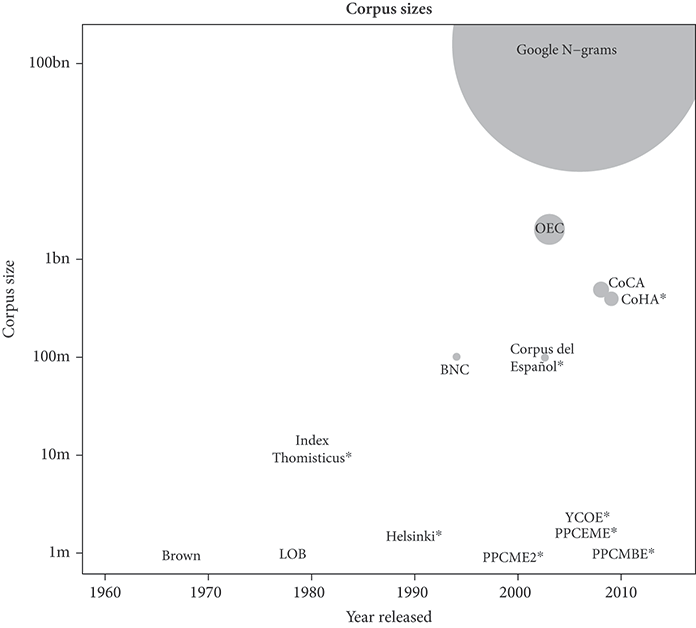
\includegraphics[scale=0.8]{corpora}
\caption{\label{fig:corpora} Selected historical and modern, predominantly English corpora by year and size, image from \citet{quantitative-historical}.}
\end{figure}

\subsubsection{Computational Historical Linguistics and Corpus Linguistics}
\label{subsubsec:comphist-corpus}

One prominent and conventional way of utilizing computational methods in historical linguistics, which is simultaneously highly relevant to this thesis, is for quantitative, corpus-based inquiries. As \citet{gillivray_2023} note, corpus-based research and quantitative research in this field have been on the rise in recent years. \citet{quantitative-historical} also present a framework for working with historical data quantitatively. They highlight that these methods are often pioneered by people interested in the new technology that is available and in ways to apply it to historical linguistics. It is therefore difficult to define the field of computational historical linguistics as anything other than the overlap between the methods and tools utilized in a variety of computational fields and historical data. \citet{quantitative-historical} argue strongly in favor of well-annotated corpora, highlighting the importance of not only thorough content annotation but also the inclusion of metadata. They note that in the case of manual annotation, strict guidelines should be enforced, and mention automated annotation as a promising field --- although historical data does present various issues for such an approach, especially when the tools used are not well-adapted. \autoref{fig:corpora} illustrates the size disparity between selected, mostly English, modern and historical corpora, highlighting the possible need for more historical data in this format. A more extensive historical corpus can be, for example used to automatically detect and track collocations and their development, as well as other changes \citep{garcia-garcia-salido-2019-method}.

\subsubsection{Syntactic variation}
\label{subsubsec:syntactic-var}

Another interesting computational approach, implemented by \citet{johannsen-etal-2015-cross}, pertains to assessing variation in syntax. The authors gather data from speakers from varying backgrounds, tag it using state-of-the-art dependency parsers and POS taggers, and extract subtrees representing relations between different POS tags present in the data. The authors conduct an analysis of a selection of most prominent relations and compare the differences between groups of speakers based on e.g. their age and gender. While the authors of this paper focus on the variation between users of a language based on age and gender, this approach could likely be implemented for diachronic studies as well. According to the authors, this method allows for a larger amount of data to be analyzed than traditional sociolinguistic methods. A simplified version of this method, using only part-of-speech tags, is utilized in \autoref{subsec:ngrams}; however, that simplification removes the possibility for a comparison of the results to those from the paper. It also makes it impossible to observe long-distance dependency relations.

\subsubsection{Part-of-speech tagging of historical data}
\label{subsubsec:historical-pos-tagging}

One more area that could be said to be balancing between NLP and (computational) historical linguistics is part-of-speech tagging of historical data. Research of this kind is conducted for a variety of reasons: on the one hand, evaluating the way in which taggers adapted to modern data perform on historical data can help improve the tools and pre-processing procedures themselves, and on the other hand, the ability to accurately tag data using automated tools, as mentioned in \autoref{subsubsec:comphist-corpus}, is highly relevant for the creation of corpora. 

\begin{table*}[h]
\begin{center}
\begin{tabular}{|l|cccc|}
\hline \bf Paper & \bf Language & \bf \makecell[c]{Modern Text \\ Accuracy (\%)} & \bf \makecell[c]{Historical \\ Test Data \\ Accuracy (\%)} & \bf \makecell[c]{Preprocessed \\ Historical \\ Test Data \\ Accuracy (\%)} \\ \hline
\citet{rayson07} & English & 96 & 82--88.5\% & 89--93.2\% \\
\citet{scheible11} & German & - & 69.6\% & 79.7\% \\
\citet{bollmann-2013-pos} & German & - & 23--81.8\% & 83.4--95.6\% \\
\citet{hupkes16} & Dutch & 96 & 60\% & 92\% \\
\citet{adesam-bouma-2016-old} & Swedish & 94.2\footnotemark & 45\% & 70\% \\
%\citet{waszczuk2018morphosyntactic} & Polish &  - & \makecell[c]{precision and recall: \\ 88.3--90.3\%\\88.3--90.3\%} & - \\
\hline
\end{tabular}
\end{center}
\caption{\label{table:others-tagging-results} Test results on modern, historical, and preprocessed historical data in other experiments. Note: these experiments used different kinds of taggers, tagsets, pre-processing methods, and data, which means that their results are not fully comparable.}
\end{table*}
%\footnotetext{Naturally, the taggers were not tested on the same modern text, as they are tools for different languages, therefore, the results are not fully comparable.}
\footnotetext{Here the tagger was trained on historical data as well.}

\autoref{table:others-tagging-results} presents a variety of studies where various taggers, predominantly trained on modern data, were tested on historical data, with and without preprocessing. Not included in the table is \citet{waszczuk2018morphosyntactic}, as the measures that they do not provide accuracy as a measure, but instead use precision and recall (both around 88.3\% for baroque texts and 90.3\% for texts from 1830--1918). They also do not utilize any preprocessing procedures. However, this study is highly relevant to the topic of the thesis as not only does it tackle Polish, but also tests one of the taggers tested in the subsequent sections. 

\subsubsection{Data normalization vs. variation}
\label{subsubsec:normalization-var}

% dipper-waldenberger-2017-investigating
A number of papers concerning historical NLP and the application of modern tools to historical data highlight the improvements that the normalization of e.g. spelling or punctuation can yield to the performance of various tools and that a requirement for normalization is imposed by many available tools \citep{rayson07, scheible11, bollmann-2013-pos, hupkes16, adesam-bouma-2016-old, garrette-alpert-abrams-2016-unsupervised, estarrona-etal-2020-dealing, hamalainen-etal-2021-lemmatization}. However, \citet{dipper-waldenberger-2017-investigating} point out that the mapping of different variants in historical data to their modern counterparts that occurs in such preprocessing can be very informative as far as language variation and change is concerned. Using the normalized forms as a way to establish which historical word-forms are equivalent, the authors conduct a diatopic mapping of language variation in historical German. Additionally, they group and analyze the so-called "rewrite rules" for normalization by area and conduct an analysis to reveal what kinds of variation it is mitigating, such as morphological, phonological, or graphemic variation, indicating that these are the kinds of differences that can be inferred from the word-forms themselves. Findings presented by \citet{eisenstein_variation} support the claim that orthographic variation can be motivated phonologically, while simultaneously showing that the extent to which a new variant becomes widespread can depend on e.g. the word form or a specific meaning. 

\subsubsection{Tool adaptation}
\label{subsubsec:tool-adaptation}

% regnault-etal-2019-challenges - important because I do not do this syntactic annotation for n-grams
% % sanchez-marco-etal-2011-extending
Another solution when it comes to using existing tools for nonstandard data is adapting the tools themselves instead of normalizing the data. For instance, as far as syntactic annotation of historical data is concerned, \citet{regnault-etal-2019-challenges} highlight that there still is a need for adapting the existing tools if high performance is to be achieved. In their research they adapt a metagrammar in order to be able to automatically annotate Old and Middle French texts. Alternatively, \citet{sanchez-marco-etal-2011-extending} argue that extending a tool's dictionary and retraining it with a small corpus leads to very good results on nonstandard data, as illustrated by their experiments on historical Spanish; additionally, they conduct an error analysis of the remaining problematic tokens in order to establish the ways in which their method improved the tool's performance.

\subsubsection{Modelling language change and dialectical variation}
\label{subsubsec:modelling}

% zampieri-etal-2016-modeling, peirsman_geeraerts_speelman_2010, donoso-sanchez-2017-dialectometric, hovy-purschke-2018-capturing
In another approach, \citet{zampieri-etal-2016-modeling} attempt to model language change in historical Portuguese using word and POS n-grams as features for SVM classification of the source texts in terms of the date of publication; while they conclude that the latter are not as informative, they conclude that they can provide some insights in later analysis. They also note that the larger the word n-grams, the worse the performance, and that the opposite is true for POS n-grams. Looking at lexical variation, \citet{peirsman_geeraerts_speelman_2010} attempt to use computational methods to retrieve cross-lectal synonyms and identify lectal markers with Belgian and Netherlandic Dutch corpora and resources as data; while their methods are successful at identifying some differences, they are still hindered by polysemy and the colloquial status of some of the words. In an investigation into the modern dialects of Spain, \citet{donoso-sanchez-2017-dialectometric} approximate the difference in dialects using cosine similarity and the Jensen-Shannon metric; however, they still rely on a lexical database to select which concepts to target in their comparison. While \citet{hovy-purschke-2018-capturing} utilize Doc2vec to obtain document representations for German and, together with geographical information, form clusters corresponding to dialect areas, this method does not appear to report what kind of variation is identified. 

\subsection{Computational background}
\label{subsec:algorithms}

Although their use in this thesis is discussed in more detail in \autoref{sec:exp-setup}, relevant algorithms and architectures are introduced in this subsection. It is important to note that this thesis does not attempt to improve any of these, but instead tests how they can be utilized in similar inquiries. 

\begin{figure}[H]
\centering
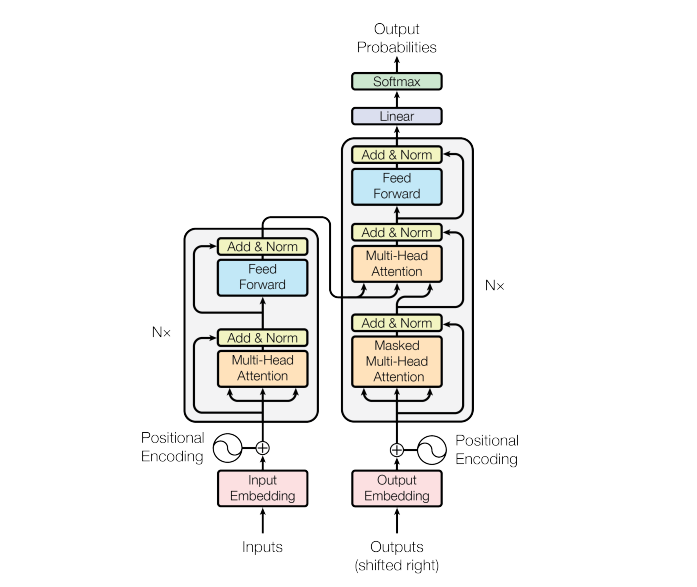
\includegraphics{transformers}
\caption{\label{fig:transformers} The architecture of a transformer model, image from \citet{vaswani2017attention}.}
\end{figure}

Within this thesis, a selection of pre-trained tools is used. These include Morfeusz2 and Concraft-pl, as described in \cite{waszczuk-2012-harnessing} and \citet{kie:wol:17:morf}, the Stanza neural pipeline, outlined in \citet{qi2020stanza}, and University of Sheffield's UPOS tagger \citep{gatecloud}. In addition, two pre-existing tagger architectures are trained on selected data. These include a pipeline provided by \citet{wolf-etal-2020-transformers} for utilizing any of the HuggingFace BERT-like models (in the case of this thesis it was BERT for Polish) \citep{kłeczek_2021}. These harness the power of the so-called transformer neural model architecture (as depicted in \autoref{fig:transformers}), first introduced by \citet{vaswani2017attention}, which employs attention to determine which elements should weigh in on the result; this allows the model to better take into account which elements of the sentence can indicate the appropriate tag, in addition to the information from the word representation. The other trainable tagger architecture is Marmot, an improved Conditional Random Fields-based tagger, using what authors call "pruned CRFs." This approach consists of "[creating] increasingly complex lattices and to [filtering] candidate states at every step to prevent a polynomial increase in lattice size" \citep{mueller-etal-2013-efficient}. The method for this is presented in \autoref{fig:marmot}. It is worth noting that neither of these algorithms has been implemented from scratch, and openly available implementations are used in this thesis, and the use of all of these tools is specified in \autoref{sec:exp-setup}. 

\begin{figure}[H]
\centering
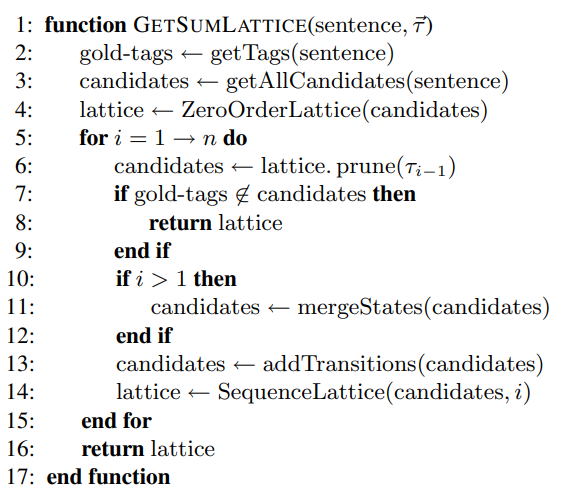
\includegraphics[scale=0.6]{marmot}
\caption{\label{fig:marmot} A mock-algorithm for CRF pruning, image from \citet{mueller-etal-2013-efficient}.}
\end{figure}

In addition, this thesis makes use of a number of existing libraries for Python 3 and their implementations of various algorithms and measures, such as the evaluation measure calculations provided by \citet{scikit-learn} or data structures from \citet{reback2020pandas}. 

\newpage

\section{Experimental Setup}
\label{sec:exp-setup}

This section contains a description of both the data and the experiments that were conducted. The entirety of the code, alongside unannotated and annotated data, is provided in \autoref{app-resources}. The results of the experiments are presented and discussed in \autoref{sec:results}. A description of the data and the annotation process is provided in \autoref{subsec:data} and \autoref{subsec:annotation}. Generally, the experiments can be divided into three categories: tagger and lemmatizer testing (\autoref{subsec:bert-tagging}, \autoref{subsec:marmot-tagging}, \autoref{subsec:stanza-tagging}, \autoref{subsec:morfeusz-tagging}, \autoref{subsec:ud-tagging}, with the error analysis detailed in \autoref{subsec:error-annotation}), n-gram statistics (\autoref{subsec:ngrams}), and investigations into the National Corpus of Polish (\autoref{subsec:nkjp-vocab}). 

\subsection{Data}
\label{subsec:data}

The data used in the experiments originates from a memoir penned by Juliusz Czermiński in 1899 in Rzeszów. The original manuscript is preserved in the collection of Zakład Narodowy im. Ossolińskich (also known as Ossolineum) with the signature 15374/II, according to the library's catalog, but cannot be accessed digitally \citep{ossolineum}. At some point in the past, typewriter copies of the manuscript (possibly made from another copy and not the original manuscript) have been made and distributed among the author's descendants. In recent years, one of them, Piotr Kociat\-kiewicz, undertook the effort of copying over the text into a Word file, and it is this digitalized data that was used throughout the thesis. Unfortunately, due to the time constraints and the physical difficulty of accessing the manuscripts, no assessment of the quality of the transcription could be made.

As mentioned before, the data originates from one author and belongs to the genre of memoir. The author was a native of an area that encompasses nowadays south-eastern Poland and western Ukraine but was not independent at that time, and instead a part of the Austro-Hungarian Empire following the partitions of the Polish–Lithuanian Commonwealth in the late 18\textsuperscript{th} century. From what can be gathered from the contents of the memoir, the author considered himself to be Polish and wrote in an idiolect closely resembling the Polish language. However, due to the text's age and region of origin, it is likely that it diverges from standard modern Polish with regard to spelling (from which pronunciation may be inferred), grammar, and vocabulary. This assumption is strengthened by the fact that following the periodization of the history of Polish as outlined by \citet{długosz-kurczabowa_dubisz_2006}, the text could be classified as an example of writing in "early" New Polish (npol. 1.), which diverges from Modern or "late" New Polish (npol. 2.).
%% maybe this should be written elsewhere? but where?
%% add stuff from the other book once I unpack it

Both the relative understandability of the text to a native speaker of Polish and the potential for it to differ from standard Polish make it a good candidate for inquiries into how potential differences between a historical text and a modern standard could be identified computationally. It is, nevertheless, worth keeping in mind that this text need not be representative of Polish in general at the time of its writing and this thesis should be regarded as an investigation of this particular memoir and its author's language, not of late 19\textsuperscript{th} century Polish at large.

The entirety of the memoir consists of 37 405 tokens, according to Microsoft Word's word count functionality. Out of those, the first 360 sentences, corresponding to 10 286 tokens, were manually annotated with UPOS (universal part of speech) tags, and the first 115 sentences, corresponding to 3271 tokens, were additionally annotated with XPOS (language-specific part of speech) tags and lemmas following the tagsets used by \citet{wroblewska-2018-extended} in PDB (Polish Dependency Bank), which itself is the largest UD corpus available for Polish, and therefore conforms to the UD format. This decision was made due to the accessibility and universality of these tagsets, and because the results could then be compared to PDB's test set; additionally, some other tools, while not trained on PDB, seemed to be using the same tagset. The details of the annotation process are discussed in \autoref{subsec:annotation}. While this means that only roughly more than a quarter of the text was annotated with the UPOS tags and less than a tenth with the XPOS tags and lemmas, the annotation of the entire text was deemed to be beyond the scope of this thesis, especially given the complicated nature of the XPOS tags and the fact that the annotation had to be of high quality. Additionally, small test samples are not unheard of when it comes to tagger-related experiments using historical data \citep{bollmann-2013-pos, hupkes16, rayson07}. 

\begin{figure}[h]
\centering
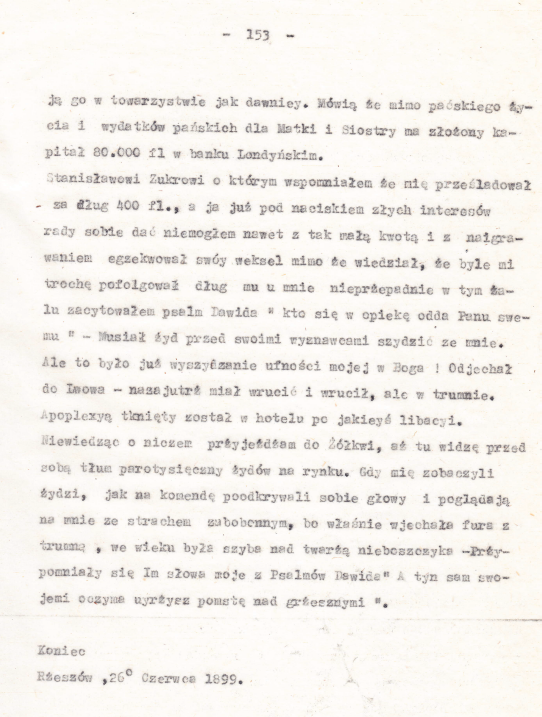
\includegraphics[scale=0.8]{memoir}
\caption{\label{fig:memoir} The final page of the typewriter transcription of the original text of the memoir, from which the digital copy was made. Private collection. Image courtesy of Anna Chodorowska.}
\end{figure}

Simultaneously, most of the procedures described in the subsequent subsections were also conducted on the PDB (Polish Dependency Bank) corpus, so that the results could be compared to those obtained on modern data; additionally, some of the taggers were locally trained on the PDB train set. As mentioned before, PDB is the largest UD-style treebank available for Polish. It features 22 152 sentences consisting of a total of 347 377 tokens, annotated according to the UD guidelines in the CoNLL-U format. Aside from the lemmas, UPOS, and XPOS tags, which are utilized in this project, the treebank also features an annotation of syntactic relations between words \citep{wroblewska-2018-extended, universaldependencies}.

Another corpus utilized in this thesis is the National Corpus of Polish, a large collection of Polish texts that the authors claim to be balanced and representative of the language. While the entirety of the corpus is not available to be downloaded due to copyright issues, there do exist search engines for it, and a small subcorpus is available for downloading. This subcorpus is manually annotated with a tagset closely resembling the UD XPOS tags \citep{nkjp}. Within this project, only one of the search engines is directly utilized, although other tools may rely on data from this corpus \citep{pęzik_2012}.

In the initial stages of the project, there was an idea to compare the results obtained from the discussed data with results from running the same experiments on a subset of the Korba Corpus, also known as The Electronic Corpus of 17th and 18th c. Polish Texts (up to 1772) \citep{korba}. Although code allowing for the extraction of the desired data from the corpus files was developed for the needs of this thesis, it was later discovered that not only does the corpus not include UPOS tags, but its XPOS-like tags differ in small but relevant ways from the ones used in PDB. Finding a way to unify these tagsets was deemed to be beyond the scope of this thesis and the Korba Corpus was not used in later experiments. 

\subsection{Data Annotation}
\label{subsec:annotation}

The process of data annotation occurred in a number of steps. First, the data was converted from a \texttt{.docx} file to a \texttt{.txt} file and segmented so that every line corresponded to a paragraph or a section in the original text. This served as a basis for the first major step in the annotation, namely the manual annotation of a selected subsection of the text with UPOS tags. Subsequently, Python code in the form of a Jupyter Notebook that allowed for the pre-tagging using the Morfeusz morphological analysis tool \citep{kie:wol:17:morf} in tandem with Concraft-pl \citep{waszczuk-2012-harnessing, waszczuk2018morphosyntactic}, a morphosyntactic tagger which relies on Morfeusz's analyses was developed (these two tools are discussed in more detail in \autoref{subsec:morfeusz-tagging}). This was used for pre-annotating the subset of the data that was intended to be annotated with XPOS tags and lemmas, as those were the types of annotation provided by Morfeusz and Concraft-pl. The results, along with the UPOS tags, were outputted into a \texttt{.conllu} file which adhered to the standards of that format. This pre-annotation was then manually reviewed and corrected wherever necessary.

As mentioned in \autoref{subsec:data}, the tagset used for this task was the same as the one used in the Polish Dependency Bank, the largest of the UD-standard treebanks for Polish \citep{wroblewska-2018-extended}. That was also the corpus that was consulted in problematic cases; whenever necessary, an online dictionary of the Polish language was consulted as well \citep{pwn_n.d.}.

Each type of tagging (lemma, UPOS, XPOS) was characterized by its own difficulties. When it comes to manual lemmatization --- the task that would appear to be the easiest, at least to a native speaker --- the issue was deciding what lemmas to enter for words that were spelled in an unconventional way. A number of the words in the text were spelled together in ways that are not permitted by standard Polish; other words were simply spelled using a different spelling convention or in a way that possibly reflected pronunciation. A decision was made to preserve these peculiarities, while simultaneously trying to present the word in its base form, in an attempt to infer the idiolectal base form. For example, \textit{oyca} `(of the) father' was lemmatized to \textit{oyciec} instead of \textit{ojciec} `father', which would have been the modern spelling. This was done in order to preserve the original spelling of the words and reflect how the author would have likely written the base form of the word. In addition, in one of the experiments which consisted of comparing the vocabulary of the text with that of a modern Polish corpus (discussed in more detail in \autoref{subsec:nkjp-vocab}), preserving the original spelling was essential, as one of the goals of the comparison was to determine if words and lemmas with that spelling occur in the corpus. It is, nevertheless, important to note that this decision may have negatively impacted the lemmatization performance of some tools during evaluation. 

UPOS tags, which not only reflect the approximate word class but sometimes also the role of a word in the sentence, have proven to generally be rather straightforward to assign. Nevertheless, there were some instances of words that could be classified as more than one class without a straightforward way to differentiate between those two supposed meanings. One such example is the word \textit{około} 'around,' which could be classified as either an adposition or a particle in the treebanks - and for which the Dictionary of the Polish Language provided two practically identical definitions, that did not allow for an easy distinction between the two \citep{okolopwn}. Another problematic category was the rule that verbs normally treated as auxiliaries should be classified as regular verbs in purely existential sentences \citep{polishud}. 

Finally, the XPOS tags required the most attention during the review of the preannotation, predominantly due to the fact that oftentimes they include a lot of information about the features of the token, such as gender, number, aspect, etc. Consequently, there was not much room left for token-level ambiguity, but issues stemming from syntactic ambiguity persisted. Another major issue throughout the annotation process was determining whether a verb-derived word should be classified as a gerund/participle or as a noun or adjective. For example, \textit{bombardowanie} 'bombing' could be treated either as a noun or as a gerund of the verb \textit{bombardować} 'to bomb.' If the word was attested for in PDB, it was tagged in the same fashion as in the corpus. Otherwise, the decisive factor was the presence of the derived form as an independent word in a dictionary.  

\subsection{Experiment 1: BERT XPOS and UPOS-tagging}
\label{subsec:bert-tagging}

The first experiment consisted of fine-tuning a BERT model for a token classification task. Being able to fine-tune one's own model was beneficial, as one was in full control of the data and tagset used in the process. However, that cannot be said for the data utilized in the training of the original BERT model. 

The fine-tuning and evaluation were conducted using the code and instructions provided in the Transformers library for Python in \texttt{transformers/examples/legacy/token-\\classification/}, with minor changes meant to adapt the procedure to the provided data  \citep{wolf-etal-2020-transformers}. Preprocessing of both the training, evaluation, and testing data was modified to include another script, \texttt{preproc\_bert.py}, which removed the lines required by the CoNLL-U format for Polish for non-split tokens (i.e. situations where an element that the UD requires to be described separately is attached to another word, for instance \textit{słyszałem} `I heard' is required to be split into \textit{słyszał}, the l-participle of the verb meaning `to hear' and \textit{em}, the "mobile inflection" indicating the person). These lines do not feature any annotation but indicate the range of original word. Therefore, they were irrelevant for the tagging, and could actually be disruptive if left in the text. No other major changes were made to the settings of the fine-tuning, as the goal of this experiment was not to find the best hyperparameters for the task, and the suggested hyperparameters were assumed to be acceptable.

The model used as a basis for the fine-tuning was \texttt{bert-base-polish-cased-v1} by \citet{kłeczek_2021}. While both the cased and uncased versions of the model perform well on different evaluation tasks, according to the author the cased model features improvements over the uncased one. Additionally, due to the historical data featuring unconventional capitalization and many proper names, it was deemed relevant to maintain the capitalization.

A total of two models were fine-tuned, one for UPOS-tagging, and one for XPOS-tagging. They were trained, evaluated, and tested on the PDB data. Subsequently, both of the models were tested on the historical data, which was pre-processed in the same fashion as the PDB data. The results were automatically saved in \texttt{.txt} files. Although this process did output a selection of evaluation measures, for the sake of comparability, those were recalculated in a Jupyter Notebook file using functions from \texttt{functions.py}, a Python file containing functions used across several different experiments, both for the modern and historical test set, with the evaluation measures' implementation from Scikit-learn and various pandas elements \citep{scikit-learn, reback2020pandas, mckinney-proc-scipy-2010}. A number of \texttt{.xlsx} files containing all of the annotations and only the erroneous ones were created for later analysis.  

\subsection{Experiment 2: Marmot XPOS and UPOS-tagging}
\label{subsec:marmot-tagging}

The next experiment similarly consisted of training a tagger architecture on PDB data. In this case, the tagger was a CRF-based framework called Marmot \citep{mueller-etal-2013-efficient}. Although Marmot does have pre-trained models for Polish, their tagsets did not appear to be compatible with the one used in this thesis. Therefore, a new model was trained on the PDB training set, and tested on both the PDB test set and the historical data. Just as in \autoref{subsec:bert-tagging}, this data had to be preprocessed using \texttt{preproc\_bert.py}. Marmot can be trained to tag both UPOS and XPOS simultaneously, so only one model was trained. 

Marmot does not output any evaluation measures, so the results were imported into a Jupyter Notebook and the necessary measures were calculated there. Same as before, the results were also output in the form of two \texttt{.xlsx} files, one for all the results and one including just the mistakes made by the tagger.

\subsection{Experiment 3: Stanza XPOS-tagging, UPOS-tagging, and lemmatization}
\label{subsec:stanza-tagging}

Another tagging service that was used to annotate the historical data was that provided by Stanza \citep{manning-etal-2014-stanford, qi2020stanza}. Stanza's neural pipeline provides all three desired functionalities: lemmatization, XPOS annotation, and UPOS annotation. The default package for the Polish language in Stanza is based on PDB, which was extremely convenient as the tagsets were certain to match if no changes were introduced while constructing the package. In order to obtain the annotations, the Stanza pipeline was run in a Jupyter Notebook environment on both the modern and historical data. Measures compatible with those from other experiments were output for every category, and \texttt{.xlsx} files containing all of the annotation and the errors were produced for later comparison. In addition, measures and results were produced for the comparison of lowercased gold standard and lowercased output of lemmatization, as it has been observed that Stanza returns all the lemmas in lowercase.

\subsection{Experiment 4: Morfeusz XPOS-tagging and lemmatization}
\label{subsec:morfeusz-tagging}

Unlike the previously tested taggers, this one relies on two complementary tools. Morfeusz is a morphological analyzer, which provides both the possible morphological analyses of input tokens and their lemmas. This is done on the basis of provided linguistic data. In the case of this experiment, and for the sake of compatibility with the other tool, the SGJP data, based on a Grammatical Dictionary of Polish was selected \citep{sal:etal:15, kie:wol:17:morf}. In order to disambiguate Morfeusz's predictions, another tool, Concraft-pl is used. Similarly to Marmot in \autoref{subsec:marmot-tagging}, it is a CRF-based tool. The pre-trained model that is provided and that is compatible with the aforementioned version of Morfeusz has been trained on data from the National Corpus of Polish \citep{nkjp, waszczuk-2012-harnessing, waszczuk2018morphosyntactic}. While these tools have not been based on or trained on PDB, the tagset that their use appears to be compatible with the XPOS tagset of PDB. This divergence in terms of source data is naturally something that should be taken into account when comparing the results from different taggers. Nevertheless, the matching tagsets make these tools a relevant addition to the project. 

In this experiment, the pipeline designed for the pre-annotation of the historical data using Morfeusz and Concraft-pl, organized within a Jupyter Notebook file, was modified to obtain the predictions based on the input from the \texttt{.conllu}, not \texttt{.txt} file, as before. Naturally, the desired output format was also changed, as the results of the tagger experiments were not saved in \texttt{.conllu} files. Since this combination of tools does not have the option to introduce custom tokenization, an algorithm matching misparsed tokens to their gold standard counterparts had to be developed. Once again, as far as lemmatization was concerned, measures were obtained both with the original capitalization and with both the gold standard and the predictions being lowercased, so that a comparison between different tools' performance when it comes to lemmatization could be made, as the other one investigated within this thesis has proven to return results solely in lowercase. Similarly to the experiments with other taggers, the list of all tokens and annotations was saved for both XPOS tags and lemmas in the form of an \texttt{.xlsx} file, along with similar spreadsheets containing only the errors that the tools have made.

\subsection{Experiment 5: UD Cloud UPOS-tagging}
\label{subsec:ud-tagging}

The final tagger used in this project is a maximum entropy model based on the GATE Learning Framework plugin hosted by the University of Sheffield \citep{gatecloud}. This tagger was trained on the Polish corpora available in UD, including PDB. This tagger, called the "UD tagger" in this thesis, only provides UPOS tags for the input tokens. One of its severe limitations is the daily quota that makes it impossible for large amounts of data to be processed at once, which meant that the PDB test data had to be tagged in batches. Despite these shortcomings, the tagger was still deemed worthy of inclusion, as it is also based, at least in part, on PDB, and provides tagging that is compatible with the tagset used in this project, and simultaneously the architecture of this tagger differs from the other ones used.

The tagging process was conducted via the provided API, from a Jupyter Notebook file. As mentioned before, the way the data was fed to the tagger was dictated by the practical constraints of a daily limit imposed on the tagger. Therefore batches of sentences were fed to it, and, in the case of the PDB test set, the whole set had to be split for the tagging process. Analogously to the case of Morfeusz and Concraft-pl (see \autoref{subsec:morfeusz-tagging}), this tagger tokenizes the text on its own, meaning that some elements may end up misparsed in comparison to the manual tokenization, and a similar algorithm was used to single out these elements and assure that the output list from the tokenizer was of the same length as the input, with 1:1 correspondence between the elements. Same as with the other taggers, both the output and only the erroneous tags were saved to \texttt{.xlsx} files.

\subsection{Experiment 6: n-gram statistics}
\label{subsec:ngrams}

Following \citet{johannsen-etal-2015-cross}'s method of approximating a language user's syntax by means of obtaining "treelet" statistics, i.e. statistics of subtrees in the UD-style dependency relation trees, an attempt was made at developing a similar method, albeit perhaps less informative when it comes to long-distance relations. While \citet{johannessen-etal-2020-comparing} did use automatic pre-annotation, \citet{regnault-etal-2019-challenges} suggest that in case of historical data such tools might need adapting. Due to a manual revision of pre-annotation using non-adapted tools being deemed too time-consuming for this project, the closest subunits that could be obtained for the data were n-grams over the XPOS and UPOS tags. As previously mentioned, this method may hopefully reveal insights into close-distance dependencies or trends in word order but fails at taking into account long-distance relations. Nevertheless, differences between the sentences in PDB's test set and the historical data in question in terms of these statistics could hint at larger syntactic differences.

The statistics were obtained from the manually annotated \texttt{.conllu} files and the PDB test set with Python code within a Jupyter Notebook. N-grams were constructed with functions using NLTK tools and displayed and saved to \texttt{.xlsx} files using pandas \citep{bird_loper_klein_2009, reback2020pandas, mckinney-proc-scipy-2010}. For both kinds of data and POS annotation unigrams, bigrams, and trigrams were constructed and counted, with both the raw numbers and the relative frequencies provided. The relative frequencies of given n-grams were also compared side by side for the modern and historical data.

\subsection{Experiment 7: National Corpus of Polish vocabulary comparison}
\label{subsec:nkjp-vocab}

The final investigation into the historical data itself consisted of assessing in what ways its vocabulary differs from that of modern Polish. To this end, an API access to the National Corpus of Polish was used \citep{pęzik_2012}. Access to the most recent version of the API was provided upon request by Dr. Pęzik. 

Vocabulary comparisons were conducted in a Jupyter Notebook file for both PDB's test set and the historical data, on tokens as well as lemmas. All of the search settings were kept except for a narrowing of the search range in terms of time, balance, and limit. The limit variable determined how many detailed hits were returned out of all the matches. This information was not very relevant, as the goal of the search was only to determine whether or not the word occurs in a given subsection of the corpus. Therefore this was reduced from the default setting of 20 to 1. The balance setting determines whether the search is conducted in a balanced subcorpus or across all the texts. Since the search was intended to verify whether a word is attested for in the corpus, it was found that a larger selection of text would be preferable, despite it being unbalanced. The time range for the source texts was narrowed down to 1945 until 2023. While the memoir was written at a time that is considered to be the tipping point between the first and second period of New Polish, the experiments conducted within this thesis were intended to compare it with modern Polish \citep{długosz-kurczabowa_dubisz_2006}. Therefore, some other, more recent cutoff point had to be selected, keeping in mind the fact that the selection of texts in the corpus should still be representative of all of the language. The decision was made for 1945 to be that cutoff point, as that date marked the end of the Second World War and the most recent change to Poland's borders.\footnote{Alternatively, 1989, the year that Poland's communist government fell and the country underwent a transformation, was considered, but was deemed too recent}

The results were retrieved both for tokens in their original form and for the lemmas; in the latter case, a special search syntax was used, where \texttt{lemma**} is intended to return all the possible inflectional forms for the word. Raw numbers and a relative proportion of the words not found in the corpus were obtained, and all of the unique tokens or lemmas for the historical data were saved in \texttt{.xlsx} files alongside their counts in the aforementioned subcorpus. The code also printed out a list of the items that were not found in the National Corpus of Polish. Finally, a qualitative inspection of the items that were not found in the corpus was conducted, alongside a comparison of the historical ones with a lexicon of words typical for Borderlands Polish provided in \citet{kurzowa_1983}. 

\subsection{Tagging and lemmatization error annotation}
\label{subsec:error-annotation}

Since a major part of the experiments consisted of testing various taggers on modern and historical data, it was decided that a joint error analysis should be conducted. Since the goal of the thesis is not to verify which tagger is the best or what kind of errors particular types of taggers tend to make, this kind of analysis was considered warranted, as it would reveal which tokens were consistently problematic across the different tools, and not what types of errors a particular tagger tended to struggle with.

The error analysis was conducted in three steps. First, a Jupyter Notebook file was created in which the lists of the results for different lemmatizers (Stanza, Morfeusz), XPOS taggers (Stanza, Morfeusz, BERT, Marmot), and UPOS taggers (Stanza, BERT, Marmot, UD) were combined and tokens for which at least two tools provided a wrong tag were extracted. For the lemmatizers that meant that all of the tools had to make a mistake while tagging the data, while for the POS taggers only half of them had to be wrong. This eliminated errors that stemmed purely from a certain tagger's tendency to misclassify some tokens unless that tendency was shared by more than one tool. Those errors were then saved into three separate \texttt{.xlsx} files. In the second stage, the errors were manually annotated depending on the subjectively perceived possible cause of the error. Each category (lemmatization, XPOS, UPOS) received a slightly different set of error types due to apparent differences in what tokens were problematic, but a number of error types persisted cross-categorically. Finally, annotated \texttt{.xlsx} files were loaded into a second Jupyter Notebook, and counts and relative frequencies for each error type were calculated. 


\newpage

\section{Results and Discussion}
\label{sec:results}

% LEMMATIZATION
\subsection{Lemmatization}
\label{subsec:lemmatization}

%% should I cite here too?
As outlined in \autoref{subsec:stanza-tagging} and \autoref{subsec:morfeusz-tagging}, the two lemmatization tools that were used in this thesis were Stanza and Morfeusz. The only evaluation measure that was obtained for lemmatization was accuracy, as lemmatization differs from other classification problems in terms of the sheer number of possible classes, and therefore other measures were considered superfluous. \autoref{table:lemmas} depicts the accuracy per model and per type of test data. What is immediately visible is Morfeusz's better performance on both modern and historical data. One potential explanation, that Stanza handles the input text worse than Morfeusz, has mostly been refuted by an inspection of the errors that both lemmatizers made and the fact that this tendency is consistent regardless of the type of data. Many of the mismatches between the gold standard lemma and the assigned lemma in the case of Stanza was due to Stanza returning all lemmas in lowercase by default, meaning that had capitalization been disregarded in this task, Stanza could have reached a higher accuracy score, both for modern and historical data.  \\

\renewcommand{\arraystretch}{1.25}
\begin{table}[h]
\begin{center}
\begin{tabular}{|cc|c|}
\hline \bf Model & \bf Data & \bf Accuracy \\ \hline
\multirow{2}{4em}{Stanza}
& PDB & 90.89\%  \\
& memoir & 83.49\%  \\
\multirow{2}{4em}{Morfeusz}
& PDB & 97.77\%  \\
& memoir & 91.01\% \\ 
\hline
\end{tabular}
\caption{\label{table:lemmas} Lemmatization accuracy per model and per test data type.}
\end{center}
\end{table}

Another noticeable difference is the significantly worse performance of the taggers on the historical data when compared to the modern data. The qualitative error analysis conducted on tokens that were mislabelled by both of the lemmatizers\footnote{This allowed for the elimination of errors caused by tagger-specific issues and made it possible to focus on instances where it was more likely that it was the token itself that was problematic; for instance, this eliminated nearly all of the instances where Stanza returned a lowercase lemma where it was not expected to do that.} revealed characteristics of the mislabelled tokens that could be identified by a human annotator. The error statistics can be seen in \autoref{table:lemmas-errors}, and explanations and examples of the specific error types can be found in \autoref{table:error-type-explanations} in \autoref{error-types}. Two major categories that can be distinguished from among the errors are the spelling-related ones and foreign vocabulary ones. The first category encompasses \textit{y}, \textit{e}, \textit{nie}, capitalization, abbreviation\footnote{This category does not include `spelling' as that error type is reserved for typos, while this overarching category is intended to gather tokens that are intentionally spelled in an unconventional way.}, while the latter - proper name, surname, name, foreign, archaic. Those two categories also appear to be rather text-specific, as the potentially unique vocabulary and a specific non-standard way of spelling are not features of the Polish language in general, but of the writing of this particular author. Naturally, there still are errors that stem from typos or ambiguities, but the bulk of the issues appear to be connected to the text's peculiarities. Simultaneously, the problematic tokens hint at there being a need for a more uniform way of determining what lemma to choose for verb-derived nouns and adjectives or words that have more than one acceptable spelling.

\renewcommand{\arraystretch}{1.25}
\begin{table}[h]
\begin{center}
\begin{tabular}{|c|cc|}
\hline \bf Error Type & \bf Raw Freq. & \bf Relative Freq. (\%) \\ \hline
\textit{y} & 35 & 24.14\%  \\
proper name & 30 & 20.69\%  \\
\textit{nie} & 19 & 13.10\%  \\
spelling & 12 & 8.28\% \\ 
surname & 12 & 8.28\% \\
capitalization & 8 & 5.52\% \\
abbreviation & 8 & 5.52\% \\
\textit{e} & 7 & 4.83\% \\
ambiguous & 3 & 2.07\% \\
name & 3 & 2.07\% \\
unidentified & 3 & 2.07\% \\
problematic & 2 & 1.38\% \\
foreign & 2 & 1.38\% \\
archaic & 1 & 0.69\% \\
\hline
\end{tabular}
\caption{\label{table:lemmas-errors} Types of errors and their raw and relative frequencies among the historical tokens that were mislabelled by both Stanza and Morfeusz.}
\end{center}
\end{table}

While a major drawback of this method of discovering a historical text's peculiarities is that there needs to be a gold standard to compare the performance of the lemmatizers to, it does reveal some interesting insights into the kinds of tokens that appear to be nonstandard for Polish and typical for a given text. What could be done in case of texts with no gold standard is simply reviewing the entire output - but that would, in the long run, be almost identical to manually lemmatizing it in the first place.

% UPOS
\subsection{UPOS-tagging}
\label{subsec:upos-tagging}

As detailed in \autoref{subsec:bert-tagging}, \autoref{subsec:marmot-tagging}, \autoref{subsec:stanza-tagging}, and \autoref{subsec:ud-tagging}, the four taggers that either utilized or could be trained to utilize the UD tagset were BERT, Marmot, Stanza, and the UD Cloud tagger. Unlike in the case of lemmatization, when it comes to tagging, there is a specific number of classes in question, which allowed for the extension of the evaluation metrics from just accuracy to accuracy, weighted precision, weighted recall, and Matthew's Correlation Coefficient, which are presented in \autoref{table:upos}. Since the UD tagset is not large, precision and recall were also calculated for each class for a deeper insight into which classes are the most problematic \citep{ud-tagset}. These results can be found in \autoref{upos-class-measures}. Based on the general evaluation measures BERT performed best on both the modern and the historical dataset, while the UD Cloud tagger has the worst performance on both of the test sets. Although not by a lot, Stanza's neural pipeline outperforms Marmot. For all of the taggers the historical dataset achieves a consistently lower score than the modern one, indicating issues that are not specific to the taggers themselves. 

\renewcommand{\arraystretch}{1.25}
\begin{table}[H]
\begin{center}
\begin{tabular}{|cc|cccc|}
\hline \bf Model & \bf Data & \bf Accuracy & \bf Precision & \bf Recall & \bf MCC \\ \hline
\multirow{2}{4em}{BERT}
& PDB & 99.20\% & 99.20\% & 99.20\% & 99.08\% \\
& memoir & 94.50\% & 94.72\% & 94.50\% & 93.77\%  \\
\multirow{2}{4em}{Marmot}
& PDB & 97.73\% & 97.75\% & 97.73\% & 97.38\% \\
& memoir & 90.61\% & 90.79\% & 90.61\% & 89.30\% \\
\multirow{2}{4em}{Stanza}
& PDB & 98.40\% & 98.41\% & 98.40\% & 98.16\% \\
& memoir & 93.31\% & 93.52\% & 93.31\% & 92.43\% \\
\multirow{2}{4em}{UD Cloud}
& PDB & 90.98\% & 91.17\% & 90.98\% & 89.59\% \\
& memoir & 83.41\% & 84.12\% & 83.41\% & 81.17\% \\ 
\hline
\end{tabular}
\caption{\label{table:upos} UPOS-tagging evaluation measures (accuracy, precision (weighted), recall (weighted)), Matthew's Correlation Coefficient per model and per test data type. Although calculated, F1 is not given since it can be calculated from precision and recall. Per class precision and recall can be found in \autoref{upos-class-measures}}
\end{center}
\end{table}

Similarly as in the case of lemmatization, manual annotation of errors made by the taggers has revealed certain recurring features, as outlined in \autoref{table:pos-errors}; this time, however, the token in question did not have to be misclassified by all of the taggers, and instead only two of them had to have made a mistake while tagging a given token, as that was deemed more likely to still remove the tagger-specific issues while preserving more information on the possible problematic features of the data than if all of the taggers had to misclassify the token. A more detailed definition of the types of errors along with examples can be found in \autoref{table:error-type-upos-explanations} in \autoref{error-types}.

Similarly to the errors made during lemmatization, the errors can be divided into spelling-related and foreign vocabulary-related. However, another category appears to be taking shape here, namely that of form-related errors. These encompass a number of ambiguous, ending, problematic, and impersonal type errors, with the category of "ambiguous" being the most numerous error category in general. In that case the word itself appears to be classified according to the wrong meaning or just by the ending, which can itself be ambiguous and lead to different interpretations. Clearly, the word form itself (or the inflectional ending itself) should not be the only factor determining a word's class; this may hint at an additional level of difficulty in terms of unusual word order if such information is utilized by the tagger. In addition, some errors stem from the UD tagging rules which are complicated e.g. when it comes to the VERB vs. AUX distinction for the verb \textit{być} in Polish. What is worth noting is the high number of capitalization-related errors. It appears that capitalization is factored in as a feature when it comes to tagging words as PROPN - and, as a result, regular words written unexpectedly with a capital letter at the start are often misclassified as such. 

\renewcommand{\arraystretch}{1.25}
\begin{table}[H]
\begin{center}
\begin{tabular}{|c|cc|}
\hline \bf Error Type & \bf Raw Freq. & \bf Relative Freq. (\%) \\ \hline
ambiguous & 208 & 21.80\% \\
capitalization & 199 & 20.86\% \\
\textit{y} & 109 & 11.43\%  \\
unidentified & 62 & 6.50\% \\
archaic & 59 & 6.19\% \\
UD & 58 & 6.08\& \\
surname & 41 & 4.30\% \\
\textit{e} & 41 & 4.30\% \\
\textit{nie} & 28 & 2.94\% \\
ending & 24 & 2.56\% \\
spelling & 23 & 2.41\% \\
proper name & 21 & 2.20\% \\
problematic & 20 & 2.10\% \\
digits & 17 & 1.78\% \\
foreign & 13 & 1.36\% \\
uncommon & 12 & 1.26\% \\
abbreviation & 11 & 1.15\% \\
impersonal & 4 & 0.42\% \\
name & 2 & 0.21\% \\
currency & 1 & 0.11\% \\
special & 1 & 0.11\% \\
\hline
\end{tabular}
\caption{\label{table:pos-errors} Types of errors and their raw and relative frequencies among the historical tokens that were mislabelled by at least two of four UPOS taggers (BERT, Marmot, Stanza, UD Cloud).}
\end{center}
\end{table}

Class-specific measures yield a deeper insight into which classes in particular are more problematic. For BERT (as can be seen in \autoref{table:bert-pr}), all of the classes in the modern text, with the exception of INTJ and SYM perform very well. The two aforementioned classes could be problematic due to their scarcity. They are also not present at all in the historical data. As for the memoir, there is a noticeable drop in performance for ADV, AUX, PART, PROPN, SCONJ, and X - which are also less numerous than some of the other classes. Additionally, there is possibly some confusion between AUX and PART when it comes to the classification of the token \textit{to} `it' or `is'. Naturally, the numerous new proper nouns found in the historical text are also problematic, not to mention the issue of nonstandard capitalization. 

Marmot (\autoref{table:marmot-pr}) similarly struggles with SYM and INTJ in the modern data, but it also scores relatively lower on AUX, PART, PROPN, and X on the PDB test set. When it comes to the historical data, a noticeable drop in performance can be noticed for the ADJ category, alongside ADV, AUX, PART, PROPN, SCONJ, and X. Aside from the ADJ category (which is more complicated due to place name-derived adjectived being capitalized by the author and surnames being misclassified as adjectives), the same categories seem to be problematic for Marmot as for BERT, although in this case some of these issues are already noticeable on the modern test set.

Stanza's results (which can be found in \autoref{table:stanza-pr}) show high precision, but low recall on the problematic INTJ and SYM classes. Otherwise the tagger performs quite well across all of the categories in the modern data, with the possible exception of relatively low recall on PART. When it comes to the historical data, a noticeable drop in performance can be observed for ADJ, AUX, PROPN, SCONJ, and X, which again mostly overlaps with the categories that were problematic for the aforementioned taggers.

The UD Cloud tagger (\autoref{table:ud-pr}) shows a much more varied performance across the classes on both the modern and historical test data. As far as the PDB test set is concerned, it struggles with ADJ, ADV, AUX, NUM, PROPN, and X classes in particular. As for the memoir, a large drop in performance can be observed for most classes. Noticeably, the tagger performs well on ADP, CCONJ, and PUNCT, and has a high precision, but very low recall on DET. While the issues that this tagger has with the modern data do oartly overlap with the classes that were problematic for other taggers, this tendency is not that clear on the historical data due to the overall bad performance of the tagger. However, the issues visible on the PDB test set may hint to these classes being more problematic in both modern and historical data, and perhaps the errors made while classifying those are more visible due to the classes' lowqer frequencies.

Although there is an overlap in terms of what features can lead to a token being misclassified, they seem to be of different importance when it comes to assigning UPOS tags compared to lemmatization. UPOS tagging does share the same issue as lemmatization when it comes to the need for some gold standard to compare the tagging to. While it does hint at certain text-specific issues, such as nonstandard spelling or unusual vocabulary, the bulk of the errors appears to stem from the ambiguity of some tokens.

% XPOS
\subsection{XPOS-tagging}
\label{subsec:xpos-tagging}

In accordance with what was described in \autoref{subsec:bert-tagging}, \autoref{subsec:marmot-tagging}, \autoref{subsec:stanza-tagging}, and \autoref{subsec:morfeusz-tagging}, the four tools used for XPOS-tagging experiments were BERT, Marmot, Stanza's neural pipeline and the combination of the morphological analyzer Morfeusz and a morphosyntactic tagger Concraft-pl. All of these tools were previously used for either lemmatization or UPOS tagging. While the same general evaluation measures as in UPOS-tagging were employed in this task, a decision was made to leave out the tag-specific measures due to the sheer number of possible classes. The possible labels for the fine-tuned BERT model, extracted from the training and test set of PDB along with the historical data, consist of 898 different classes. 

The overall performance of the tools in the XPOS-tagging task was worse than in the UPOS-tagging one. This could be attributed to a larger number of classes that require finer distinctions to be made. Same as before, all of the tools perform noticeably worse on historical data compared to the modern data. The best performing tool on both test sets is BERT, and the worst - Marmot. What is worth pointing out in this case though is that Morfeusz and Concraft-pl's CRF architecture does outperform Stanza's neural pipeline slightly, but only on modern data.  

\renewcommand{\arraystretch}{1.25}
\begin{table}[H]
\begin{center}
\begin{tabular}{|cc|cccc|}
\hline \bf Model & \bf Data & \bf Accuracy & \bf Precision & \bf Recall & \bf MCC \\ \hline
\multirow{2}{4em}{BERT}
& PDB & 95.65\% & 95.13\% & 95.65\% & 95.47\% \\
& memoir & 89.39\% & 89.75\% & 89.39\% & 89.05\%  \\
\multirow{2}{4em}{Marmot}
& PDB & 89.27\% & 88.95\% & 89.27\% & 88.83\% \\
& memoir & 80.22\% & 81.34\% & 80.22\% & 79.60\% \\
\multirow{2}{4em}{Stanza}
& PDB & 94.29\% & 94.25\% & 94.29\% & 94.05\% \\
& memoir & 87.68\% & 88.44\% & 87.68\% & 87.28\% \\
\multirow{2}{4em}{Morfeusz}
& PDB & 94.43\% & 95.36\% & 94.43\% & 94.20\% \\
& memoir & 84.26\% & 86.83\% & 84.26\% & 83.76\% \\ 
\hline
\end{tabular}
\caption{\label{table:xpos} XPOS-tagging evaluation measures (accuracy, precision (weighted), recall (weighted)), Matthew's Correlation Coefficient per model and per test data type. Although calculated, F1 is not given since it can be calculated from precision and recall.}
\end{center}
\end{table}

A manual error analysis and annotation has revealed a number of trends concerning the mistakes that the taggers make, as presented in \autoref{table:xpos-errors}. Definitions and examples of the errors can be found in \autoref{table:error-type-xpos-explanations} in \autoref{error-types}. A similar trend can be noticed in terms of the kinds of errors as in the UPOS-tagging task. The most numerous error type is the ambiguous errors, where one word form corresponds to multiple possible tags (e.g. in some declension paradigms certain cases have the same form). Once again, the prevalence of this errors hints either at the taggers not being able to properly utilize the contextual information that is necessary for the disambiguation of the class either due to their architecture or to the text's unusual word order; and again, the latter cannot be fully concluded simply from these results. 

One error category that is relatively prominent, namely digits, appears to stem from the tools utilizing different strategies when it comes to numbers written as digits. Some of them classify them as \textit{dig}, while others attempt to provide the tag as if the number were written out with letters. Another tagset-related issue is that of currency mistakes; the XPOS tagset generally divides masculine nouns into three subgenders: m1, which includes animate human nouns, m2, which includes animate non-human nouns, and m3, which includes inanimate nouns. These are supposed to reflect which form the determiner \textit{który} `which' takes when referring to that noun \citep{ud-masculine-gender}. According to this, however, there are less obvious words that belong to the m2 category, such as currency names, which did seem to pose a problem for the taggers. In general, some mistakes were made when distinguishing between the m1 and m3 category for other tokens as well, but they were not classified separately.

Finally, although not numerous, two kinds of errors are worth mentioning in the context of the data, namely the gender and vocative ones. Although the gender category partly overlaps with the aforementioned masculine subgender disctinction, a number of the instances in this error category stem from the fact that not all personal pronouns in Polish reflect gender (the first and second person in both singular and plural do not have an overt marking of the gender on the pronoun itself). However, since some do, all of the personal pronouns are annotated for gender. This leads to a number of personal pronouns being misclassified as masculine, when they should, in fact, be feminine, as they are uttered by a female character and followed by feminine verb or adjective forms. As for the vocative category, when the word can be interpreted otherwise, the taggers tend to not utilize the tags for the vocative case. Both of these issues hint at the fact that the training data used for the taggers may be lacking in dialogues where both first and second person personal pronouns and nouns in the vocative case would be more present. Additionally, the tendency to select masculine over feminine for the pronouns may hint at a potential gender bias in the data.

\renewcommand{\arraystretch}{1.25}
\begin{table}[H]
\begin{center}
\begin{tabular}{|c|cc|}
\hline \bf Error Type & \bf Raw Freq. & \bf Relative Freq. (\%) \\ \hline
ambiguous & 199 & 38.20\% \\
unidentified & 65 & 12.48\% \\
proper name & 52 & 9.98\% \\
\textit{y} & 39 & 7.49\% \\
digits & 25 & 4.80\% \\
problematic & 22 & 4.22\% \\
\textit{nie} & 20 & 3.84\% \\
spelling & 18 & 3.46\% \\
archaic & 17 & 3.26\% \\
foreign & 16 & 3.07\% \\
surname & 12 & 2.30\% \\
uncommon & 10 & 1.92\% \\
currency & 8 & 1.54\% \\
\textit{e} & 7 & 1.34\% \\
gender & 4 & 0.77\% \\
vocative & 3 & 0.58\% \\
abbreviation & 2 & 0.38\% \\
name & 2 & 0.38\% \\
\hline
\end{tabular}
\caption{\label{table:xpos-errors} Types of errors and their raw and relative frequencies among the historical tokens that were mislabelled by at least two of four XPOS taggers (BERT, Marmot, Stanza, Morfeusz).}
\end{center}
\end{table}

The issues that plague the XPOS taggers resemble those characteristic of UPOS tagging, with some novel types of errors being more indicative of the issues with the tagset or the training data. Once again, while this method does hint at unusual vocabulary and spelling practices being present in the text, and allows for the noticing of patterns within those trends, it requires prior manual annotation, which makes it more difficult to utilize it at a larger scale.

% ngrams - tomorrow
\subsection{n-gram statistics}
\label{subsec:ngram-stats-results}

% nkjp
\subsection{NKJP vocabulary comparison}
\label{subsec:nkjp-comparison-results}

As discussed in \autoref{subsec:nkjp-vocab}, a comparison of the unique tokens and lemmas from both of the test sets against a subsection of the data from the National Corpus of Polish was conducted. As visualized in \autoref{table:nkjp-results}, noticeably more tokens and lemmas from the historical data were not found in the National Corpus of Polish when compared to the results from the PDB test set. The difference is statistically significant. 

\renewcommand{\arraystretch}{1.25}
\begin{table}[H]
\begin{center}
\begin{tabular}{|cc|c|c|c|}
\hline \bf Data & \bf Data & \bf Total unique & \bf Not found & \bf \% \\ \hline
\multirow{2}{4em}{PDB}
& lemmas & 7583 & 44 & 0.58\%  \\
& tokens & 12601 & 56 & 0.44\%  \\
\multirow{2}{4em}{Historical}
& lemmas & 1213 & 86 & 7.09\%  \\
& tokens & 4302 & 346 & 8.04\% \\ 
\hline
\end{tabular}
\caption{\label{table:nkjp-results} Raw and \% numbers of tokens and lemmas unique to the modern or historical test sets when compared with a subset of the NKJP.}
\end{center}
\end{table}

An inspection of the items that were returned as having no matches in the National Corpus of Polish for the PDB test set (which can be found in the resources in \autoref{app-resources}) reveals that many of them overlapped across the lemma and token category (i.e. if a token was not found in the corpus, neither was its lemma, and vice versa). A number of the missing items include punctuation, which appears to not be included in the corpus searches, as well as different numbers and numerals, which, due to their practically infinite number, is understandable. Additionally, a number of place names, names, surnames, and brand names were not found in the NKJP. Finally new borrowings with nonstandard spelling reflecting the original pronunciation (the dimunitive \textit{lajwik} `live (stream)') as well as highly specialized vocabulary (\textit{trichlorobenzen} `trichlorobenzene') were not found in the National Corpus of Polish either, which is warranted as these are either new or very rarely used words.

A similar trend in terms of both the token and the lemma missing from the National Corpus of Polish can be noticed for the historical data, although here the comparison is more difficult, as the unique tokens were extracted from a larger text sample than the unique lemmas (which had to be manually annotated). Once again, some punctuation is listed as not found due to the search engine's limitations. However, almost no standard numbers or numerals are listed as not found, with the exception of \textit{cwansiger} `20 (coin/bill)', which appears to be a borrowing from German. Similarly as with the modern data, a large number of proper names and surnames was not found in the corpus. A large part of the vocabulary with no hits in the NKJP consists of either words spelled in a nonstandard fashion (with the spelling of \textit{nie} together with the verb it modifies and the use of the grapheme \textit{y} for /j/ being the most prominent; there is one interesting instance of the sound \textipa{/\textrtailz/} being spelled as \textit{rż}, while the two accepted modern spellings are \textit{rz} and \textit{ż}\footnote{These two spellings reflect a past phonemic merger.}), or of words that appear to be out of use or highly specific to the sociohistorical context of the text (such as \textit{mandatariat} `the position of being a potentiary' or \textit{mortyfikować} `to self-flagellate'), with a potential overlap between the two categories. What is also noticeable is that some of the words reappear with multiple variations of spelling (e.g. \textit{jurysdykcya}, \textit{juryzdyksya} `jurisdiction' or \textit{mandataryusz}, \textit{mandatyrusz} `potentiary') indicating a certain degree of inconsistency when it comes to spelling.

A simple comparison of the vocabulary of a given text or dataset to that of a large corpus of a given language appears to yield informative results as far as those texts' divergence from the standard is concerned. With the exclusion of terms that are naturally unlikely to appear in the corpus (surnames, proper names), there still remain tokens and lemmas that were not identified in the corpus due to their spelling or rarity, and some of the same conclusions as to the nature of these differences can be drawn here as from the experiments \autoref{subsec:lemmatization}, \autoref{subsec:upos-tagging}, and \autoref{subsec:xpos-tagging}. While this method does not return as many items that were not found (or, in case of the taggers, errors), it only requires the text to be lemmatized, not annotated for the part of speech - and even simply searching for the tokens, and not their lemmas, yields interesting results that are not extremely different from those for lemmas. Overall, this kind of a comparison appears to be quite rewarding for the amount of preprocessing or annotation required.

\newpage

\section{Ethical Considerations}
\label{sec:ethicalcons}

Ethical concerns are ever-present within the field of Natural Language Processing. As \citet{hovy-spruit-2016-social} point out, these concerns can revolve both around the data itself and the impact that NLP can have on the society. \citet{stochastic-parrots} point out the environmental impact of computationally-heavy processes (such as training very large language models) and draw the readers' attention to how biases existing in the training data can impact the aforementioned models. A number of different tools and resources were utilized in this thesis, and many of them deserve to be discussed from an ethical point of view.

To begin with, the experiments conducted as a part of this thesis did not involve training of any large models from scratch - and the most computationally expensive part was the fine-tuning of two BERT-based part-of-speech taggers. While training a large transformer model like BERT is definitely impactful, its ability to be fine-tuned for different applications eliminates the need to train another costly model from scratch. Utilizing pre-existing, optimized code for token tagging suited for this model likely streamlined the process as well. With the exception of Marmot, the training of which does not appear to be computationally expensive, the other taggers were already pre-trained, which made this investigation much more justifiable than training many models from the start would be with the environmental impact in mind. 

While a lot has been written about different biases in NLP, \citet{blodgett-etal-2020-language} find that many such discussions are "vague, inconsistent, and lacking in normative reasoning." They adopt a division of biases into allocational, meaning ones where the system bias distributes some resources unfairly to some social groups, and representational, where some groups are misrepresented or omitted by the system. The authors present recommendations for future work with bias in NLP, and while some of them are not relevant to this thesis, their suggestion to explicitly state what behaviors and what kinds of biases exist in the system or the data, how they could be harmful, and to whom, is of high importance. One instance of a representational bias displayed by the tools tested in this thesis has been described in \autoref{subsec:xpos-tagging}. According to the UD XPOS annotation, the first- and second-person singular pronouns are annotated for gender despite not overtly displaying it. During the tagging process, the tools did annotate pronouns used by a female speaker as masculine. This kind of a system behavior could be harmful if displayed at a larger scale, as it disregards the presence of women as speakers - depending on what this tagging is used for in a downstream task, this could lead to e.g. a dialogue system addressing its interlocutor using incorrect pronouns and forms. 

Biases in large language models and other NLP tools do not necessarily stem from the code itself. As \citet{garimella-etal-2021-intelligent} note, "unstructured data often contain several biases, and natural language processing (NLP) models trained on them learn and sometimes amplify them." It is therefore important to discuss the kinds of data used in this thesis and whether or not they can contain such biases (potentially leading to the aforementioned gender representation bias). The author of the Polish version of BERT, \citet{kłeczek_2021}, points out that the data used to pre-train his models may include biases and stereotypes, and, consequently, these could be visible in downstream tasks. While the National Corpus of Polish is claimed to be balanced and representative of the language at large, its creators do not address the issue of biases, and one can assume that certain prejudices can be reflected in the texts that constitute the corpus \citep{nkjp}. While, as \citet{wroblewska-2018-extended} explains, the Polish Dependency Bank is largely based on the National Corpus of Polish, it does include sentences from other sources, and a similar conclusion can be drawn about this dependency bank as about the NKJP. As far as the historical data discussed in this thesis is concerned, it is likely to contain biases, as it only comes from one author. As pointed out in \autoref{subsec:ngram-stats-results}, in comparison with the PDB, the author of the memoir uses proportionally more masculine animate human nouns, potentially leading to an over-representation of men at the cost of other genders, a bias that could be amplified had this data been used to train a tool for later use.  

Another tangentially related issue worth considering in the light of this thesis is the representation of small languages or dialects and the regional and diachronic variation in NLP. \citet{mcenery-etal-2000-corpus}, \citet{soria-etal-2016-fostering}, as well as  \citet{hovy-2018-social} point out that the lack of corpus data for such languages severely impedes the development of appropriate NLP tools, which can, in turn, lead to some social groups being excluded from utilizing such tools or result in their language becoming more endangered. While the data analyzed in this thesis is not a sample of a modern minority language or dialect, some of the methods tested in the experiments could be used for exploring contemporary language variation as well, potentially contributing to solving this issue. 

Finally, while both the out-of-context sentences provided in PDB and the limited access that users have to the texts that constitute the National Corpus of Polish are methods for dealing with copyright and privacy issues, working with an independently transcribed and annotated text may pose its own ethical problems. However, in the case of this thesis the data in question is historical, and its author has passed away around a century ago, which largely voids the issue of the author's consent for the use of his text. 





\newpage

\section{Critiques and Limitations}
\label{sec:critiques}

While certain limitations of this thesis project have already been mentioned in previous sections, it is worthwhile to summarize them and discuss other potential issues. The first few of those pertain to the data itself, as outlined in \autoref{subsec:data}. While the original manuscript is available physically at a library in Poland, the version of the data utilized in this project has been first transcribed from the manuscript on a typewriter, and then from the typewriter version into a \texttt{.docx} file. This introduces possibilities for transcription errors, making the data less reliable than if it were transcribed directly from the manuscript. 

Another kind of limitation related to the data could be that it only comes from one author and is not very large. However, the aim of this thesis was to explore this particular memoir, not the entirety of late 19\textsuperscript{th}-century Polish. One issue connected with this is that, consequently, the genre of the memoir and of the texts featured in the PDB are not necessarily the same, and some of the differences may stem not from language variation at large, but from this genre mismatch. While it is relevant to keep in mind that this data is not very representative, this limitation does not necessarily invalidate the thesis project.

Finally, the project would have greatly benefitted from all the experiments being run on an additional sample of older historical data. Unfortunately, due to differences in the tagsets, the Korba Corpus could not be used. While results for historical data do exist for one of the taggers, this unfortunately meant that the other tools' performance on the memoir in question could not be compared to older data, and thus the effectiveness of the methods could not be judged based on such a comparison.

As far as the annotation is concerned (\autoref{subsec:annotation}), the limited time and womanpower available meant that only a part of the data could be annotated. Ideally, this annotation should be proofread by another trained native speaker, but, unfortunately, that was not possible within the given timeframe. This is likely to have negatively impacted the quality of the annotation. Additionally, as discussed in \autoref{subsec:ngram-stats-results}, including the syntactic dependency annotation could have yielded more interesting results; once again though, the choice to omit this annotation was made due to aforementioned reasons. On the topic of annotation, one of the limitations of many of the discussed methods is that they require the historical data to already be annotated. However, those methods could also point in the direction of what kind of pre-processing would be needed for a more reliable automated annotation of historical data.

While the performance of BERT-based taggers was outstanding, it is possible that it could have been better. As described in \autoref{subsec:bert-tagging}, the hyperparameters used to fine-tune the taggers were the ones suggested by default by the authors of the tagging framework. It is possible that these were not fully optimal for the task.

The error annotation (\autoref{subsec:error-annotation}) conducted in this project is largely subjective, and some of the categories are partly overlapping. Some tokens could likely be classified as more than one category. It is important to keep in mind that this annotation was not intended to yield a strict measure, but to offer more general insights into what kinds of tokens are the most problematic for the taggers and lemmatizers.

Finally, as discussed in more detail in \autoref{subsec:ngram-stats-results}, the time limitations made it impossible to analyze and discuss all of the obtained n-gram results. The number of possible XPOS tags is staggering, and the decision to construct n-grams out of them without clustering them into more general categories resulted in output that was too large to analyze in the allotted time. 

\newpage

\section{Future Work}
\label{sec:futurework}

A number of the issues mentioned in \autoref{sec:critiques} could be better addressed had the scope of the project been wider and had it been possible to allot more time to it --- and it is some of these discarded ideas that form the basis of the potential future work. 

As far as the memoir itself is concerned, completing the annotation thereof with lemmas, UPOS, and XPOS tags would have constituted a small but valuable contribution to the body of annotated historical Polish. It would also have been interesting to see this data with full UD-style annotation, including dependency relations. Furthermore, the library where the manuscript is held appears to be in possession of some of the correspondence by the same author, which could be similarly transcribed and annotated; the memoir's digital version could also benefit from being compared to the contents of the manuscript to eliminate potential transcription errors.Following what has been said in \autoref{subsubsec:tool-adaptation}, it might be worth it to try to adapt existing tools for better automatic annotation when it comes to extending the scope of the annotation of this data. 

Including more of the data and a fuller annotation could potentially reveal more kinds of variation that may not be evenly distributed within the text. The presence of dependency relation annotation would enable the use of the methods implemented by \citet{johannsen-etal-2015-cross} for a higher-quality analysis of the syntax of the memoir. Refining the methods for utilizing n-gram counts, especially when it comes to the XPOS tags, could yield new insights as well.

Simultaneously, such inquiries pertaining to language variation could be conducted on more data. Both older and more contemporary non-standard data, as well as, potentially, data contemporaneous to the memoir could be explored, and, perhaps, some trends could be identified. Hearkening back to the idea of including more of the author's writing, and referring back to the Korba corpus, which features 17\textsuperscript{th}- and 18\textsuperscript{th}-century texts, the construction and annotation of a diachronic corpus of Polish for a different time period or spanning a larger time period, with the use of a tagset compatible with the UD XPOS tags (if such annotation were to be included) could be extremely beneficial for quantitative investigations into the history of Polish. Alternatively, the focus could be put on regional variation (or on both historical and regional one), as the text discussed in this thesis does display features characteristic of a group of regional dialects. What could be particularly interesting is utilizing the various methods for modelling language variation and change discussed in \autoref{subsubsec:modelling} when it comes to e.g. various Borderlands Polish texts synchronically or diachronically. 

The experiments reveal certain issues that the tools that were tested struggled with when faced with nonstandard data. While it was not the goal of this project, it could be useful to analyze these issues and explore pre-processing or normalization methods that could be implemented if such tools were to be used for the automatic annotation of larger amounts of historical data, which could be incredibly helpful given the scarcity thereof. 

One direction in which the tagger testing could be developed could be to only review certain tokens where the tagger confidence was below some threshold. Such a method could also be utilized with no golden standard available (on unannotated data). Unfortunately, this idea could not be applied to all of the taggers utilized in this project, as not all of them return confidence scores, at least not in an obvious way. Another alternative that could eliminate the need for manual annotation would be to process the input text using multiple tools (e.g. multiple lemmatizers or part-of-speech taggers) and focus on the error annotation of tokens where the tools do not return the same kind of tag or lemma; the drawback here could be tokens that are confusing all of the tools in the same way, so there is cross-tool agreement on the tag, but it is not the correct tag nonetheless.

\newpage

\section{Conclusions}
\label{sec:conclusions}

The aim of this thesis was to explore some of the potential methods for identifying language variation in Polish on the example of a late 19\textsuperscript{th}-century memoir by Juliusz Czermiński and the ways the language of the memoir differs from modern Polish. The text was expected to differ from modern standard Polish in some ways due to its age and geographical origin. A part of the text was manually annotated with lemmas, UPOS, and XPOS tags according to the UD standards for such annotation. Subsequently, a number of experiments were conducted, where the memoir was compared to the test set of PDB-UD, the largest existing UD treebank for modern Polish. The experiments included comparing the performance of various tagging and lemmatization tools on the two sets of data, reviewing the features of the most problematic tokens, part-of-speech tag statistics analyses, and a review of which tokens and lemmas from the data are not present in a specific subsection of the National Corpus of Polish.

The results, presented and discussed in \autoref{sec:results}, show that the memoir does differ from resources that are available for modern Polish, and some major trends in terms of spelling variation (the use of \textit{y} for the /j/ phoneme, the use of \textit{e} where modern Polish features the phoneme /a/, spelling the negation of a verb together with the verb itself) are identified. A noticeable drop in performance can be observed for all three categories of annotation tools, regardless of their architecture (although some perform better than others). N-gram counts of the part-of-speech tags suggest possible word order or syntactic differences but are inconclusive. A comparison of the memoir's vocabulary reveals a number of tokens that are not present in the National Corpus of Polish in the selected timespan; while some of those are proper names, other examples show spelling and vocabulary variation. Inevitably, the methods explored in this project have their drawbacks, the major one being that most of them require the data to be annotated in some way. Simultaneously, this thesis offers a small contribution to the body of annotated historical data for Polish and advocates for the usefulness of constructing larger collections of diachronic data with annotation compatible with other large annotated corpora. One more side effect of the tagger and lemmatizer experiments is that they provide a comparison of the performance of various tools on modern data.

The experiments and the results presented in this thesis explore the ways in which existing tools for modern languages can help identify language variation in historical texts. While the presented solutions may not be perfect, they encourage further discussion and research into utilizing them for diachronic linguistics, not only for simply identifying the language variation but also as an intermediate step in the process of automatizing the annotation of historical data for the creation of larger corpora. 





\addcontentsline{toc}{section}{References}
\bibliography{anthology,personal}

\newpage
\appendix
\section{Resources}
\label{app-resources}
\newpage

\section{Error Type Definitions}
\label{error-types}
\renewcommand{\arraystretch}{1.25}
\begin{table}[H]
\begin{center}
\scalebox{1}{
\begin{tabular}{p{2cm}p{4.5cm}p{3.5cm}p{1.75cm}p{1.75cm}}
\toprule \bf Error Type & \bf Definition & \bf Example & \bf Predictions & \bf Standard\\ \toprule
\textit{y} & \makecell[l]{The grapheme \textit{y} is used \\ instead of \textit{j} to signify \\ the /j/ sound} & \makecell[l]{\textit{suchey} \\ `dry'} & suchey & suchy \\ 

\makecell[l]{proper \\ name} & \makecell[l]{Potentially unfamiliar \\ proper name token} & \makecell[l]{\textit{Bludniki} \\ `Bludniki'} & \makecell[l]{Bludnik \\ bludnik} & Bludniki  \\ 

\textit{nie} & \makecell[l]{Spelling of the negation \\ with the negated word \\ in word classes that \\ normally do not allow it} & \makecell[l]{\textit{niemają} \\ `(they) don't have'} & \makecell[l]{niemaja \\ nie} & niemieć  \\ 

spelling & \makecell[l]{A likely spelling error} & \makecell[l]{\textit{ładąn} \\ `pretty'} & ładąn & ładna \\ 

surname & \makecell[l]{Potentially unfamiliar \\ surname token}  & \makecell[l]{\textit{Polanowski} \\ `Polanowski'} & polanowski & Polanowski \\ 

capitalization & \makecell[l]{Nonstandard capitalization} & \makecell[l]{\textit{Dziedzica} \\ `of the heir'} & \makecell[l]{Dziedzic \\ dziedzica} & dziedzic  \\ 

abbreviation & \makecell[l]{The token is abbreviated} & \makecell[l]{\textit{Stan} \\ `Stan'} & \makecell[l]{Stan \\ stan} & Stanisław \\

\textit{e} & \makecell[l]{The grapheme \textit{e} is used \\ instead of another vowel \\ (commonly \textit{y})} & \makecell[l]{\textit{tem} \\ `this'} & \makecell[l]{tema \\ tem} & to \\

ambiguous & \makecell[l]{The token could have \\ more than one interpretation} & \makecell[l]{\textit{dobra} \\`goods'} & dobry & dobra \\ 

name & \makecell[l]{A potentially unfamiliar \\ first name token} & \makecell[l]{\textit{Kleosię} \\ `Kleosia'} & \makecell[l]{Kleosię \\ kleosia} & Kleosia \\

unidentified & \makecell[l]{No apparent reason} & \makecell[l]{\textit{łania} \\ `doe'} & \makecell[l]{łani \\ łanie} & łania \\

problematic & \makecell[l]{The choice of the lemma \\ is up to the annotator \\ because of two spelling \\ variants or the word \\ having been derived} & \makecell[l]{\textit{bombardowaniu} \\ `of the bombing'} & \makecell[l]{bombar-\\dować} & \makecell[l]{bombardo-\\wanie} \\

foreign & The token is foreign & \makecell[l]{\textit{Toje} \\ `-'} & \makecell[l]{Toje \\ tój} & toje \\

archaic & \makecell[l]{The token is somewhat \\ archaic or regional} & \makecell[l]{\textit{człowiecze} \\ `human'} & \makecell[l]{człowieczy \\ człowiec} & człowiek \\

\bottomrule
\end{tabular}}
\end{center}
\caption{\label{table:error-type-explanations} Types and examples of errors made by lemmatizers. The translations into English are not ideal since they do not capture all of the encoded information, such as case, gender, number.}
\end{table}
\newpage

\renewcommand{\arraystretch}{1.5}
\begin{longtable}[H]{p{2cm}p{4.5cm}p{3.5cm}p{1.75cm}p{1.75cm}}
%\begin{center}
%\begin{tabular}{p{2cm}p{4.5cm}p{3.5cm}p{1.75cm}p{1.75cm}}
\toprule \bf Error Type & \bf Definition & \bf Example & \bf Predictions & \bf Standard\\ \toprule

ambiguous & \makecell[l]{The token's meaning is \\ ambiguous} & \makecell[l]{\textit{jego} \\ `his'} & PRON & DET \\ 

capitalization & Nonstandard capitalization & \makecell[l]{\textit{Patrona} \\ `patron'} & \makecell[l]{PROPN \\ NOUN } & NOUN  \\ 

\textit{y} & \makecell[l]{The grapheme \textit{y} is used \\ instead of \textit{j} to signify \\ the /j/ sound} & \makecell[l]{\textit{móy} \\ `my'} & \makecell[l]{\\ PROPN \\ ADJ \\ VERB} & DET \\ 

unidentified & \makecell[l]{No apparent reason} & \makecell[l]{\textit{wyłącznie} \\ `exclusively'} & \makecell[l]{\\ PART \\ ADV \\ NOUN} & ADV \\ 

archaic & \makecell[l]{The token is somewhat \\ archaic or regional} & \makecell[l]{\textit{pono} \\ `supposedly'} & \makecell[l]{\\ PUNCT \\ VERB \\ PROPN \\ ADJ} & PART \\ 

UD & \makecell[l]{The token has more \\ than one possible tag \\ due to UD guidelines} & \makecell[l]{\textit{był} \\ `(there) was'} & \makecell[l]{VERB \\ AUX} & VERB \\ 

surname & \makecell[l]{Potentially unfamiliar \\ surname token}  & \makecell[l]{\textit{Ostaszewskiej} \\ `Ostaszewska'} & \makecell[l]{ADJ \\ PROPN} & PROPN \\ 

\textit{e} & \makecell[l]{The grapheme \textit{e} is used \\ instead of another vowel \\ (commonly \textit{y})} & \makecell[l]{\textit{małem} \\ `small'} & \makecell[l]{ADJ \\ NOUN} & ADJ \\ 

\textit{nie} & \makecell[l]{Spelling of the negation \\ with the negated word \\ in word classes that \\ normally do not allow it} & \makecell[l]{\textit{niechciały} \\ `(they) didn't want to'} & \makecell[l]{VERB \\ NOUN \\ ADJ} & VERB  \\ 

ending & \makecell[l]{The ending of the word \\ can be indicative of \\ more than one class} & \makecell[l]{\textit{chwała} \\ `glory'} & \makecell[l]{NOUN \\ VERB} & NOUN \\ 

spelling & \makecell[l]{A likely spelling error \\ or the lack of a space \\ or a superfluous one} & \makecell[l]{\textit{wkońcu} \\ `in the end'} & \makecell[l]{ADV \\ NOUN} & NOUN \\ 

\makecell[l]{proper \\ name} & \makecell[l]{Potentially unfamiliar \\ proper name token} & \makecell[l]{\textit{Dąbrowy} \\ `Dąbrowa'} & \makecell[l]{PROPN \\ ADJ} & PROPN  \\ 

problematic & \makecell[l]{The choice of the tag \\ is up to the annotator \\ because of two spelling \\ variants or the word \\ having been derived} & \makecell[l]{\textit{służąca} \\ `servant'} & \makecell[l]{NOUN \\ ADJ} & \makecell[l]{NOUN} \\ 

digits & \makecell[l]{The token is in digits} & \makecell[l]{\textit{1} \\ `1'} & \makecell[l]{ADJ \\ NUM} & NUM \\ 

foreign & The token is foreign & \makecell[l]{\textit{daruju} \\ `-'} & \makecell[l]{\\ NOUN \\ VERB} & X \\ 

uncommon & The token is uncommon & \makecell[l]{\textit{czółno} \\ `canoe'} & \makecell[l]{ADV \\ ADJ} & NOUN \\ 

abbreviation & \makecell[l]{The token is abbreviated} & \makecell[l]{\textit{5-cioro} \\ `five'} & \makecell[l]{\\ NUM \\ NOUN \\ MIS-\\PARSED} & NUM \\ 

impersonal & \makecell[l]{The token is an \\ impersonal verb form} & \makecell[l]{\textit{wierzono} \\ `(it was) believed'} & \makecell[l]{\\ VERB \\ ADJ \\ ADV} & VERB \\ 

name & \makecell[l]{A potentially unfamiliar \\ first name token} & \makecell[l]{\textit{Wiktorów} \\ `Wiktors'} & \makecell[l]{\\ PROPN \\ NOUN} & PROPN \\ 

special & \makecell[l]{The token is a intentionally \\ spelled in a nonstandard \\ fashion} & \makecell[l]{\textit{psipiólki} \\ `quails'} & \makecell[l]{NOUN \\ ADJ} & NOUN \\ 

currency & \makecell[l]{The token is a name \\ of a currency} & \makecell[l]{\textit{Dukatów} \\ ducats} & \makecell[l]{NOUN \\ X} & NOUN \\

\bottomrule
%\end{tabular}
%\end{center}
\caption{\label{table:error-type-upos-explanations} Types and examples of errors made by the UPOS taggers. The translations into English are not ideal since they do not capture all of the encoded information, such as case, gender, number.}
\end{longtable}
\newpage

\renewcommand{\arraystretch}{1.5}
\begin{longtable}[H]{p{2cm}p{4cm}p{1.5cm}p{3cm}p{3cm}}
%\begin{center}
%\begin{tabular}{p{2cm}p{4.5cm}p{3.5cm}p{1.75cm}p{1.75cm}}
\toprule \bf Error Type & \bf Definition & \bf Example & \bf Predictions & \bf Standard\\ \toprule

ambiguous & \makecell[l]{The token's meaning is \\ ambiguous} & \makecell[l]{\textit{parafii} \\ `parish'} & subst:sg:gen:f & subst:sg:loc:f \\ 

unidentified & \makecell[l]{No apparent reason} & \makecell[l]{\textit{Ciotka} \\ `aunt'} & \makecell[l]{\\ subst:sg:acc:m1 \\ subst:sg:nom:m1 \\ subst:sg:nom:f} & subst:sg:nom:f \\

\makecell[l]{proper \\ name} & \makecell[l]{Potentially unfamiliar \\ proper name token} & \makecell[l]{\textit{Brzeżan} \\ `Brzeżany'} & \makecell[l]{\\subst:pl:gen:n:pt \\ subst:sg:gen:n:ncol \\ subst:pl:gen:m1 \\ subst:sg:gen:m1} & subst:pl:gen:n:pt  \\ 

\textit{y} & \makecell[l]{The grapheme \textit{y} is used \\ instead of \textit{j} to signify \\ the /j/ sound} & \makecell[l]{\textit{arye} \\ `arias'} & \makecell[l]{subst:pl:acc:m3 \\ adj:pl:nom:m2:pos} & subst:pl:acc:f \\ 

digits & \makecell[l]{The token is in digits} & \makecell[l]{\textit{1808} \\ `1808'} & \makecell[l]{adj:sg:gen:m3:pos \\ dig} & adj:sg:gen:m3:pos \\

problematic & \makecell[l]{The choice of the tag \\ is up to the annotator \\ because of two spelling \\ variants or the word \\ having been derived} & \makecell[l]{\textit{oczytany} \\ `learned'} & \makecell[l]{adj:sg:nom:m1:pos\\ adj:sg:nom:m3:pos \\ ppas:sg:nom:\\\hspace{0.5cm}m1:perf:aff} & \makecell[l]{ppas:sg:nom:\\\hspace{0.5cm}m1:perf:aff} \\ 

\textit{nie} & \makecell[l]{Spelling of the negation \\ with the negated word \\ in word classes that \\ normally do not allow it} & \makecell[l]{\textit{niema} \\ `(there) \\ aren't'} & \makecell[l]{fin:sg:ter:imperf \\ subst:sg:nom:f} & fin:sg:ter:imperf  \\ 

spelling & \makecell[l]{A likely spelling error \\ or the lack of a space \\ or a superfluous one} & \makecell[l]{\textit{kończ} \\ `end'} & \makecell[l]{subst:pl:gen:n:ncol \\ subst:pl:gen:f \\ impt:sg:sec:imperf} & subst:sg:gen:m3 \\ 

archaic & \makecell[l]{The token is somewhat \\ archaic or regional} & \makecell[l]{\textit{wieleż} \\ `many'} & \makecell[l]{num:pl:acc:m3:rec \\ subst:sg:nom:m3 \\ subst:sg:nom:m1} & num:pl:acc:m3:rec \\ 

foreign & The token is foreign & \makecell[l]{\textit{Toje} \\ `-'} & \makecell[l]{subst:sg:nom:n:ncol \\ xxx \\ subst:sg:nom:m1} & ign \\ 

surname & \makecell[l]{Potentially unfamiliar \\ surname token}  & \makecell[l]{\textit{Zabilskich} \\ `Zabilscy'} & \makecell[l]{subst:pl:gen:m1 \\ adj:pl:gen:f:pos \\ subst:pl:acc:m1} & subst:pl:gen:m1 \\ 

uncommon & The token is uncommon & \makecell[l]{\textit{hoża} \\ `swift'} & \makecell[l]{adj:sg:nom:f:pos \\ subst:sg:nom:f} & adj:sg:nom:f:pos \\ 

currency & \makecell[l]{The token is a name \\ of a currency} & \makecell[l]{\textit{dukatów} \\ ducats} & \makecell[l]{subst:pl:gen:m3 \\ subst:pl:gen:m2} & subst:pl:gen:m2 \\

\textit{e} & \makecell[l]{The grapheme \textit{e} is used \\ instead of another vowel \\ (commonly \textit{y})} & \makecell[l]{\textit{któremi} \\ `(with)\\which'} & \makecell[l]{adj:pl:inst:n:pos \\ subst:pl:inst:m3 \\ subst:pl:inst:m1 \\ adj:pl:inst:f:pos} & adj:pl:inst:m1:pos \\ 

gender & \makecell[l]{The token is assigned \\ the wrong gender} & \makecell[l]{\textit{Ja} \\ `I'} & \makecell[l]{\\ppron12:sg:nom:\\\hspace{0.5cm}m1:pri \\ {}} & \makecell[l]{ppron12:sg:nom:\\\hspace{0.5cm}f:pri} \\

vocative & \makecell[l]{The vocative case is \\ not properly recognized} & \makecell[l]{\textit{Ty} \\ `you'} & \makecell[l]{ppron12:sg:nom:\\\hspace{0.5cm}m1:sec} & \makecell[l]{ppron12:sg:voc:\\\hspace{0.5cm}m1:sec} \\

abbreviation & \makecell[l]{The token is abbreviated} & \makecell[l]{\textit{śp} \\ `may his \\ soul rest \\ in peace'} & \makecell[l]{ \\ brev:pun \\ subst:sg:nom:m3 \\ subst:sg:nom:m1 \\ aglt:sg:sec:\\\hspace{0.5cm}imperf:nwok \\ {}} & brev:npun \\ 

name & \makecell[l]{A potentially unfamiliar \\ first name token} & \makecell[l]{\textit{Melchior} \\ `Melchior'} & \makecell[l]{subst:sg:nom:m1 \\ subst:sg:nom:m3 \\ subst:sg:gen:f} & subst:sg:nom:m1 \\ 

\bottomrule
%\end{tabular}
%\end{center}
\caption{\label{table:error-type-xpos-explanations} Types and examples of errors made by the XPOS taggers. The translations into English are not ideal since they do not capture all of the encoded information, such as case, gender, number.}
\end{longtable}
\newpage

\section{Extended UPOS measures}
\label{upos-class-measures}

\begin{table}[H]
\begin{center}
\scalebox{1.1}{
\begin{tabular}{|l|cc|cc|}
\hline \bf POS-tag & \multicolumn{2}{c|}{\bf Modern} & \multicolumn{2}{c|}{\bf Historical} \\
\bf {} & \bf Precision & \bf Recall & \bf Precision & \bf Recall \\ \hline
ADJ & 99.11\% & 99.55\% & 94.23\% & 93.31\% \\
ADP & 99.77\% & 99.91\% & 99.74\% & 98.74\% \\
ADV & 97.73\% & 98.44\% & 87.61\% & 89.94\% \\
AUX & 98.93\% & 98.93\% & 91.32\% & 84.03\% \\
CCONJ & 97.64\% & 97.99\% & 98.84\% & 93.92\%\\
DET & 98.82\% & 99.06\% & 94.52\% & 83.99\% \\
INTJ & 87.50\% & 70.00\% & 0.00\% & 0.00\% \\
NOUN & 99.58\% & 99.26\% & 95.47\% & 95.27\% \\
NUM & 97.06\% & 99.62\% & 98.21\% & 82.71\% \\
PART & 97.14\% & 95.12\% & 79.45\% & 84.47\% \\
PRON & 99.62\% & 99.44\% & 93.69\% & 91.09\% \\
PROPN & 95.88\% & 98.12\% & 84.07\% & 96.87\% \\
PUNCT & 99.96\% & 99.98\% & 99.59\% & 100.00\% \\
SCONJ & 98.68\% & 98.40\% & 87.91\% & 94.97\% \\
SYM & 50.00\% & 25.00\% & 0.00\% & 0.00\% \\
VERB & 99.72\% & 99.72\% & 95.42\% & 96.01\% \\
X & 95.62 \% & 91.91\% & 82.76\% & 72.73\% \\
\hline
\end{tabular}}
\end{center}
\caption{\label{table:bert-pr} BERT precision and recall per POS-tag per test set. }
\end{table}

\begin{table}[H]
\begin{center}
\scalebox{1.1}{
\begin{tabular}{|l|cc|cc|}
\hline \bf POS-tag & \multicolumn{2}{c|}{\bf Modern} & \multicolumn{2}{c|}{\bf Historical} \\
\bf {} & \bf Precision & \bf Recall & \bf Precision & \bf Recall \\ \hline
ADJ & 97.25\% & 97.71\% & 81.33\% & 84.57\% \\
ADP & 99.46\% & 99.74\% & 99.58\% & 98.99\%  \\
ADV & 95.59\% & 95.33\% & 86.83\% & 85.80\% \\
AUX & 91.67\% & 95.60\% & 85.02\% & 86.31\% \\
CCONJ & 96.17\% & 95.60\% & 97.20\% & 95.76\%\\
DET & 98.44\% & 96.93\% & 95.85\% & 74.94\% \\
INTJ & 46.15\% & 60.00\% & 0.00\% & 0.00\% \\
NOUN & 98.23\% & 98.04\% & 89.16\% & 91.16\% \\
NUM & 98.04\% & 94.34\% & 97.98\% & 72.93\% \\
PART & 93.49\% & 92.42\% & 78.39\% & 75.73\% \\
PRON & 99.05\% & 98.31\% & 90.66\% & 86.53\% \\
PROPN & 91.30\% & 94.09\% & 79.01\% & 86.20\% \\
PUNCT & 99.95\% & 99.95\% & 100.00\% & 100.00\% \\
SCONJ & 96.49\% & 96.21\% & 86.73\% & 91.96\% \\
SYM & 100.00\% & 25.00\% & 0.00\% & 0.00\% \\
VERB & 97.96\% & 97.43\% & 91.67\% & 92.73\% \\
X & 89.33\% & 86.73\% & 63.16\% & 54.55\% \\
\hline
\end{tabular}}
\end{center}
\caption{\label{table:marmot-pr} Marmot precision and recall per POS-tag per test set. }
\end{table}

\begin{table}[H]
\begin{center}
\scalebox{1.1}{
\begin{tabular}{|l|cc|cc|}
\hline \bf POS-tag & \multicolumn{2}{c|}{\bf Modern} & \multicolumn{2}{c|}{\bf Historical} \\
\bf {} & \bf Precision & \bf Recall & \bf Precision & \bf Recall \\ \hline
ADJ & 98.17\% & 98.99\% & 88.87\% & 93.85\% \\
ADP & 99.46\% & 99.91\% & 99.58\% & 99.07\%  \\
ADV & 94.58\% & 96.06\% & 91.16\% & 88.46\% \\
AUX & 95.44\% & 97.14\% & 84.70\% & 86.31\% \\
CCONJ & 95.47\% & 96.17\% & 98.14\% & 97.24\%\\
DET & 98.00\% & 98.47\% & 94.49\% & 79.58\% \\
INTJ & 100.00\% & 50.00\% & 0.00\% & 0.00\% \\
NOUN & 99.17\% & 98.70\% & 95.15\% & 93.44\% \\
NUM & 98.48\% & 98.11\% & 97.25\% & 79.70\% \\
PART & 95.01\% & 90.97\% & 93.33\% & 74.76\% \\
PRON & 98.63\% & 98.87\% & 90.08\% & 91.68\% \\
PROPN & 94.14\% & 96.51\% & 79.07\% & 91.89\% \\
PUNCT & 99.95\% & 99.95\% & 99.59\% & 100.00\% \\
SCONJ & 95.86\% & 94.61\% & 86.30\% & 94.97\% \\
SYM & 100.00\% & 25.00\% & 0.00\% & 0.00\% \\
VERB & 99.20\% & 98.66\% & 93.73\% & 94.15\% \\
X & 93.53\% & 93.53\% & 73.58\% & 59.09\% \\
\hline
\end{tabular}}
\end{center}
\caption{\label{table:stanza-pr} Stanza precision and recall per POS-tag per test set. }
\end{table}

%% rerun?
\begin{table}[H]
\begin{center}
\scalebox{1.1}{
\begin{tabular}{|l|cc|cc|}
\hline \bf POS-tag & \multicolumn{2}{c|}{\bf Modern} & \multicolumn{2}{c|}{\bf Historical} \\
\bf {} & \bf Precision & \bf Recall & \bf Precision & \bf Recall \\ \hline
ADJ & 83.86\% & 91.58\% & 66.73\% & 75.08\% \\
ADP & 96.65\% & 98.89\% & 96.18\% & 97.64\%  \\
ADV & 79.69\% & 75.89\% & 75.09\% & 64.20\% \\
AUX & 87.67\% & 82.98\% & 84.08\% & 78.33\% \\
CCONJ & 93.72\% & 87.14\% & 95.58\% & 95.58\%\\
DET & 94.64\% & 72.96\% & 94.58\% & 44.55\% \\
INTJ & 0.00\% & 0.00\% & 0.00\% & 0.00\% \\
NOUN & 90.82\% & 92.91\% & 80.08\% & 82.56\% \\
NUM & 73.62\% & 70.57\% & 77.00\% & 57.89\% \\
PART & 89.62\% & 80.69\% & 83.77\% & 62.62\% \\
PRON & 94.35\% & 94.06\% & 85.54\% & 81.98\% \\
PROPN & 83.40\% & 92.29\% & 69.77\% & 92.60\% \\
PUNCT & 99.93\% & 99.72\% & 100.00\% & 99.92\% \\
SCONJ & 88.62\% & 63.56\% & 83.81\% & 44.22\% \\
SYM & 0.00\% & 0.00\% & 0.00\% & 0.00\% \\
VERB & 89.46\% & 88.86\% & 81.64\% & 86.35\% \\
X & 52.24\% & 41.42\% & 56.60\% & 45.45\% \\
\hline
\end{tabular}}
\end{center}
\caption{\label{table:ud-pr} UD Cloud tagger precision and recall per POS-tag per test set. }
\end{table}
\newpage

\section{NKJP comparison output}
\label{app:nkjp}

Aside from counts and proportions of the tested vocabulary that could not be found in the National Corpus of Polish, specific tokens and lemmas were returned. The items listed below were not found in the selected subsection of the National Corpus of Polish. They are separated by whitespace.

\begin{itemize}
    \item \textbf{PDB lemmas:} ! ) 19:15 25-procentowy 642-65-85 9-miesięczny Arasyb Bielsko-Biała Bushill-Matthews Collridge Eija-Riitta HA-Il Hawełko III-1 IRSC IRSR Instagram Lunzie McMillan-Scott Minecraft PPE-DE Palmiak Stallarholmen Winfryd-Bonifacy Yeosol [ ajtemik antysubsydyjny bezfabularny bio-obrazowanie ciemku krio-elektronowy lajwik merozoit niekonscjentywny non-profit nudności odmaterializować podwaliny przeciwbiałaczkowy przeciwretrowirusowy tekstilandia trichlorobenzen Ździara
    \item \textbf{PDB tokens:} ! " \% ' '' ( ) , 19:15 25-procentowy 5-proc 642-65-85 9-miesięczna ; Ajtemików Bushill-Matthewsowi Collridge Eija-Riitta HA-Il III-1 IRSC IRSR Instagramie Kalkilli Lunzie Maggego McMillan-Scott Minecrafcie PPE-DE Palmiak Pirkera Stallarholmen Winfryd-Bonifacy Yeosol [ ] ajtemika bio-obrazowania celekoksybem efawirenzem krio-elektronową lajwika non-profit nukleozydowymi przeciwciałem przeciwretrowirusowego ry(d)zykować sakwinawiru tektilandia trichlorobenzenu tuńczykowymi zięciowskim – — ” „
    \item \textbf{memoir lemmas:} ! ) Asińdźka Bludniki Będowszczyazna Bęklowizna Cobary Czołhany Dochorów Dorchów Dłużanin Głowecki Kmińszczyzna Kurypów Lesniowice Muczynowska Nawarya Notiak Pierściorowski Pokasowce Ronantowizna Ruszkowizna Rypnin Rzotoławski Semiginów Siemginów Siemiginów Siemignów Strużewo Stryiskie Swieżaska Szołayska Temerowice Treterówna Treterówną Zebold abbum adlinencja assekuracya całorolny cwansiger daruju domnikalny dotacya dośmierć excentryczność generacya gymnazyum instantacya ioyciec jurysdykcya juryzdyksya kadectwo mandatariat mandataryusz mandatyrusz mojomu mortyfikować mychayłowu niepomiąć nieprzynieść obeymować obeyście ordynarya oycowski pełnłnomocnik przystoyna półgrunt półrolny rarachować separacya spaśne stayermarka submittować sukcessor sukcessorka sukcessya sukcesya szambelanic szyzmatycki treterianum ukochanomu warżyć wdokument świętej pamięci Żółtowizna
    \item \textbf{memoir tokens:}  ! ( ) , Abbum Adelunia Asińdźka Badenianką Bełszowcu Bełzkiem Bienkowskey Blizcey Bludnickey Bludnikach Bludnikami Bludniki Bodzowcu Borkoscy Bołszowcu Bołszowice Bołszowickim Będowszczyazna Bęklowizna Chyrowskiey Cobary Czołhanach Czołhany Dobrrzyńskiej Dochorowie Dominikalnym Domnikalnego Dorchów Dołputowie Dołputów Dziduszyckiego Dłużanie Dźurkowie Floyrana Galecyi Galicyiskiego Golejowskiemi Golejowskimi Gwoźdzu Głoweckiego Głuską Helnkę Horodzyńskiego Inżyniryi Jabłonoscy Jenerałówną Jędrżejowicz Kazimierzostwie Kleofasę Kmińszczyzna Knihinicz Knihiniczach Komornikostwa Komornikowej Kopestyńskich Koropacza Korytyńską Koziobrodzkiego Kołmyiskim Kołomyiskimc Kruszelnicy Kruszelnicę Krzywczas Kunaszowa Kunaszowie Kurypów Kutyszcza Kutyszczach Leboskich Lesniowic Luboscy Maksymowic Mandatariaty Mandataryusz Mandataryusza Mandatyrusza Michałoskich Mohorocie Muczynowską Mychayłowu Nawaryi Naybliższe Nieograniczały Niezabitoski Notiak Obertyńskim Ocyciec Ostaszeskiey Ostaszewskigo Oyciciec Oycowskiey Perekozach Pierściorowskim Pieścioroski Pieściorowski Pokasowce Poldzię Przebysławscy Przebysławski Przebysławskimi Puszczanki Puzyniance Rafałoska Rafałoskiej Romaszówki Ronantowizna Rudźwianach Rusoccy Ruszczewskich Ruszkowizna Rypnin Rzotoławskim Sadogurze Semiginów Separacya Siemginowa Siemiginowa Siemiginowie Siemiginów Siemignowa Simiginowskiego Sopohów Stamisaw Stojoskiego Strużewo Stryiskim Sukcesya Swieżaski Swieżaskiey Swojey Szamanowskim Szołayska Szołayskiego Tarmowiecki Tarnoscy Temerowiec Tomaszowiec Treterianum Treterowej Treterówną Wincentowey Woyniłowa Woyniłowie Woyniłowskich Woyniłów Wołczyńcu Zabilską Załęskiey Zebold adlinencjami administracyę ambicya arędujący assekuracyi asystencyą austyackie balożowaniu bronzowemi całorolni ciaśnieysze ciemnoblnd ciepłey cwansigera cywilney daruju delkatnieyszey domurowanego dotacyi doyrzałemi drugey drżew dway dwukoleśnym dystynkcy ekwipazach etykietalney excentryczności exkluzyi familiinemi foryszyc generacya generacyi gołey gymnazyum główney iOycu installacyę instantacyi jadałney jednająca jedwabney jendory jurysdykcyi juryzdyksye kadectwo kląby kochającey kollokacyi kompano kompleksya kompleksyi koniaż krzewowe kunaszowskie kupsze mandataryusza miarkmi mieycus mieyscowych mojomu mortyfikował najzabawney natarczywiey nawykręcawszy naybliższych nayjstarszego nayjświętszey naymował naymłodszą naymłodzy naypięknieyszey nayskładniey naystarsza naystarszych nayszczęśliwsze naywiększey nayznacznieyszą nibieszczeją niechwytało nieciosanemi niemiano nienosiło nieodjechał niepomięła nieprzyniósł niepsuło nierobiły niespokóy niespotkałem nieusuwały niewinem niezapalają niezostawili nieśniło normalney obedwie obeymował obeyrzeć obeyściu obliwamy obliwać obruciły oczem odchuchano okoloney ordynaryi osypami owalney ożewionemi perswazye pełnłnomocnik piurami piętnastulaty podedworem podeyrzenie policyu pomarłemi porozpuszczały poselskiey pospolitey powiena powiązanemi pruchniało prużnował przedewsią przepiurek przerodni przypiórki przystoyna próżnemi psipiólki póyść półgruntów półrolni rantuchem rarachować redukcyi roumianey ruwieśnika skończoney skrzętnem spaśnemi stancyę starszey stayermarka submittować sukcessorka sukcessorów sukcessyi swojey szambelanica szczupleyszey szczupłey szkrofuliczny szutrowany szyzmatycki sądowey teraźnieysze traktryerni troygiem ukochanomu uprzężone uprzężonym urzędowey warżenia wekslarek wojażerowi wsąsiedztwo wuyem wypiętnowaną wywruż wzorowem zachorowałł zaprzęgył zatabaczone zatrętwiał zawerbował zaymie zaymował zuchwałey zżadka Łomnickiey Łosiówną ładąn Świeżyńską śmieszney śniadey świcząc Żółtowizna – ” „
\end{itemize}




\end{document}


